% !TEX root = ../auv-thesis.tex
% Authoritative thesis source; edit this TeX file directly.
% Legacy Markdown material is reference-only and must not overwrite this file.

\chapter{分层实验验证与结果分析}

\section{实验体系、共同设置与评价口径}\label{sec:ch05-5-1}

本章按验证命题组织仿真、数字孪生、回放、台架和实物子链证据，回答前述观测、估计、决策与安全机制分别得到什么支持。为使每条结论都能追溯到具体条件，评价体系沿四个维度组织：其一是任务与终止判据；其二是场景、传感器和扰动建模；其三是同源同种子下的基线与消融；其四是定位、控制、近底安全和巡检评价指标。各小节明确标注证据层级、运行规模和适用范围，不把代码存在、原始数据、完成分析和可追溯结果混为同一证据，也不把不同层级结果拼接成一次``全面通过''。

第 2 章已经说明系统由仿真后端、通信接口、状态估计、任务决策和控制执行等模块构成，第 3、4 章则分别给出了状态估计与决策控制算法。本节不再重复这些模块的设计原理，而回答一个不同的问题：上述模块如何在实验中被组织成可重复运行、可施加受控扰动并能形成可审计证据的闭环。为此，本文把仿真实施划分为运行编排、在线闭环和证据生成三个相互解耦的部分。

\subsection{从场景配置到证据产物的实施架构}\label{sec:ch05-5-1-1}

一组实验首先由场景、随机种子、控制模式和仿真后端共同定义。场景给出海流、传感器退化与通信故障等外部条件；随机种子固定随机扰动实现；控制模式决定采用固定权重控制还是不确定性感知控制；仿真后端决定动力学与环境模型。四类输入在运行开始前冻结，并与代码版本、持续时间和通信方式共同写入本次运行的元数据。这样，后续指标不只对应一组数值，还能回溯到产生该数值的完整实验条件。

仿真实施架构各层的数据责任如下：

\begin{longtable}[]{@{}
  >{\raggedright\arraybackslash}p{(\linewidth - 6\tabcolsep) * \real{0.2500}}
  >{\raggedright\arraybackslash}p{(\linewidth - 6\tabcolsep) * \real{0.2500}}
  >{\raggedright\arraybackslash}p{(\linewidth - 6\tabcolsep) * \real{0.2500}}
  >{\raggedright\arraybackslash}p{(\linewidth - 6\tabcolsep) * \real{0.2500}}@{}}
\caption{仿真实施架构的运行层次与数据责任}\label{tab:ch05-simulation-implementation}\tabularnewline
\toprule\noalign{}
运行层次 & 主要输入 & 实施责任 & 主要输出 \\
\midrule\noalign{}
\endfirsthead
\toprule\noalign{}
运行层次 & 主要输入 & 实施责任 & 主要输出 \\
\midrule\noalign{}
\endhead
\bottomrule\noalign{}
\endlastfoot
实验编排层 & 场景、随机种子、控制模式、参数组合 & 生成独立运行上下文，完成启动前清理、配置冻结、就绪判定与定时收尾 & 运行元数据、进程日志与唯一运行标识 \\
仿真与接口层 & 控制指令、环境参数、故障配置 & 推进 PVS/HoloOcean 动力学，生成多速率传感器观测，经模拟管理设备注入时延、丢包、冻结、漂移与饱和，并按部署通信语义收发数据 & 受扰观测、独立真值流与设备遥测 \\
在线算法层 & 受扰观测、任务目标、系统健康状态 & 依次完成时空对齐、ES-EKF 状态估计、行为树任务选择、制导与控制、安全仲裁 & 状态估计、协方差、控制指令与诊断量 \\
证据生成层 & 真值流、估计流、控制流、诊断流 & 同步记录时序数据，离线计算定位、控制、安全和巡检指标，并按场景与种子聚合 & 单次指标、跨运行统计、图表与验收判定 \\
\end{longtable}

在线闭环以仿真器内部真实状态 \(\boldsymbol{x}^{\mathrm{gt}}_k\) 为起点。设 \(\mathcal{P}_b\) 为后端 \(b\) 的动力学推进算子，\(\mathcal{F}_{\mathcal{S}_j}\) 为场景 \(\mathcal{S}_j\) 对理想观测施加多速率采样、噪声和故障的算子，\(\mathcal{E}\) 为第 3 章的状态估计器，\(\mathcal{C}_m\) 为第 4 章控制模式 \(m\) 对应的决策控制链，则一次离散闭环可写为

\begin{equation}
\boldsymbol{z}_k
=
\mathcal{F}_{\mathcal{S}_j}
\!\left(h(\boldsymbol{x}^{\mathrm{gt}}_k),\boldsymbol{\xi}_k;s\right),
\qquad
(\hat{\boldsymbol{x}}_k,\boldsymbol{P}_k)
=
\mathcal{E}(\boldsymbol{z}_{0:k}),
\label{eq:ch05-closed-loop-obs}
\end{equation}

\begin{equation}
\boldsymbol{u}_k
=
\mathcal{C}_m(\hat{\boldsymbol{x}}_k,\boldsymbol{P}_k,\boldsymbol{r}_k),
\qquad
\boldsymbol{x}^{\mathrm{gt}}_{k+1}
=
\mathcal{P}_b(\boldsymbol{x}^{\mathrm{gt}}_k,\boldsymbol{u}_k,\boldsymbol{w}_k).
\label{eq:ch05-closed-loop-dyn}
\end{equation}

其中 \(s\) 为随机种子，\(\boldsymbol{\xi}_k\) 与 \(\boldsymbol{w}_k\) 分别表示观测扰动和环境扰动，\(\boldsymbol{r}_k\) 为任务参考。式\eqref{eq:ch05-closed-loop-obs}与式\eqref{eq:ch05-closed-loop-dyn}强调了实验可信度所依赖的一条关键隔离：控制器只接收受扰观测形成的估计状态 \(\hat{\boldsymbol{x}}_k\) 及其协方差 \(\boldsymbol{P}_k\)，仿真真值 \(\boldsymbol{x}^{\mathrm{gt}}_k\) 通过独立数据通道记录，仅在离线阶段作为误差计算基准，不进入在线控制回路。

本章大规模定量实验以 PVS 六自由度动力学为主后端，并采用与实物部署一致的二进制 UDP 语义连接模拟管理设备和 ROS2 决策控制栈。模拟管理设备不是简单的数据转发器：它在每个仿真周期先接收并限幅下行控制命令，再推进动力学；随后从真实状态生成各传感器的多速率采样，施加场景规定的故障与传输效应，最后编码为上行遥测。HoloOcean 保留为可替换的高保真视觉、碰撞与环境交互后端；两种后端共享上层数据契约，但其结果不在未对齐动力学参数和场景条件时直接混合统计。

\subsection{单次闭环实验的运行生命周期}\label{sec:ch05-5-1-2}

单次运行依次冻结场景、种子、模式与版本，启动并核验关键输出，按预定任务或时间窗口闭环记录，再完成写入与有效性检查。配置只在本次上下文修改；真值、估计、协方差、控制与诊断同步保存。记录非空、可解析且评价成功才计为有效，失败与缺失单列，不静默排除。批量比较使用一致的初始化、激活和收尾语义。

\subsection{多场景、多种子与消融实验的组织}\label{sec:ch05-5-1-3}

在单次运行之上，批量实验按场景集合 \(\mathbb{S}\)、随机种子集合 \(\mathbb{R}\)、控制模式集合 \(\mathbb{M}\) 和参数组合集合 \(\boldsymbol{\Theta}\) 的笛卡尔积组织：

\begin{equation}
\Omega
=
\mathbb{S}\times\mathbb{R}\times\mathbb{M}\times\boldsymbol{\Theta}.
\label{eq:ch05-experiment-space}
\end{equation}

每个组合建立独立记录与失败状态，完成运行数和有效样本数分别审计。固定权重与不确定性感知控制在同场景、同种子下成对比较，共享扰动实现。在线只记录原始时序，离线按真值评分，再跨运行聚合均值、分位数与成功比例。PVS、轻量闭环和硬件结果共享接口，但按各自模型层级解释，不混合统计。

\subsection{评价指标的数学定义与物理意义}\label{sec:ch05-5-1-4}

本文的评价指标分为定位、控制、地形跟随与电缆巡检四类。定位类指标刻画状态估计相对独立真值流的误差。设第 \(k\) 个样本的真实水平位置和估计水平位置分别为 \((x_k^{\mathrm{gt}},y_k^{\mathrm{gt}})\) 与 \((\hat{x}_k,\hat{y}_k)\)，则

\begin{equation}
\operatorname{RMSE}_{xy}
=
\sqrt{\frac{1}{N}
\sum_{k=1}^{N}
\left[
(\hat{x}_k-x_k^{\mathrm{gt}})^2
+
(\hat{y}_k-y_k^{\mathrm{gt}})^2
\right]}.
\label{eq:ch05-rmse-xy}
\end{equation}

深度均方根误差 \(\operatorname{RMSE}_z\)、圆概率误差 \(\operatorname{CEP}_{50}\) 与最大漂移量分别描述垂向平均误差、水平误差中位半径和最差时刻偏离。归一化新息平方（NIS）不依赖真值，用于检验滤波器给出的协方差是否与实际新息统计一致：标准 NIS 在模型自洽时服从自由度等于观测维数的卡方分布\cite{barshalom2001estimation}，维数归一化 NIS 的理论期望为 1。

控制类指标刻画跟踪与执行质量，包括航向、深度和横向路径跟踪误差、平均控制努力、求解失败回退比例、安全违规率，以及相邻控制向量差分的均方根

\begin{equation}
r_{\Delta u}
=
\sqrt{
\frac{1}{N-1}
\sum_{k=2}^{N}
\left\|
\boldsymbol{u}_k-\boldsymbol{u}_{k-1}
\right\|_2^2
}.
\label{eq:ch05-control-smoothness}
\end{equation}

\(r_{\Delta u}\) 越小，表示相邻指令变化越平滑；回退比例则以进入求解失败、超时或状态不可靠回退分支的控制周期数除以总控制周期数。地形跟随类指标以真实离底高度为基准，评价相对目标高度的均方根误差、最小安全裕度和波动程度；电缆巡检类指标围绕相对中心线横向偏移、路由完成率、埋深反演误差、检测连续性和行业标准验收状态展开。各指标的完整定义和数据契约见附录 A.6。

\subsection{数字孪生场景与证据生成流程}\label{sec:ch05-5-2}

\subsubsection{复杂海底电缆巡检场景构建}\label{sec:ch05-5-2-1}

仿真场景库由两层组成。第一层覆盖干净基线、四档多普勒计程仪（DVL）丢包、两档磁畸变、声呐杂波和综合压力，用于传感器与通信不确定性验证；第二层面向海缆巡检，把电缆几何、地形与埋设、声磁量测噪声和横流拆成可独立控制的原生因子，并与完整控制栈可运行的六类代理场景并存。第一层配置汇总如下，第二层的正式统计与真值和量测的隔离契约见第~\ref{sec:ch05-5-7}节（场景因子与名义强度见附录 A.1）：

\begin{longtable}[]{@{}llll@{}}
\caption{仿真场景库及扰动配置}\label{tab:ch05-scenarios}\tabularnewline
\toprule\noalign{}
场景 & 扰动类型 & 严重程度 & 用途 \\
\midrule\noalign{}
\endfirsthead
\toprule\noalign{}
场景 & 扰动类型 & 严重程度 & 用途 \\
\midrule\noalign{}
\endhead
\bottomrule\noalign{}
\endlastfoot
干净基线 & 无 & 干净环境 & 算法基线对照 \\
DVL 丢包·轻度 & DVL 丢包 & 10\% & 轻度速度观测丢失 \\
DVL 丢包·中度 & DVL 丢包 & 30\% & 中度速度观测丢失 \\
DVL 丢包·重度 & DVL 丢包 & 60\% & 重度速度观测丢失 \\
DVL 丢包·极重度 & DVL 丢包 & 90\% & 极重度速度观测丢失 \\
磁畸变·轻度 & 磁畸变 & 轻度饱和阈值 & 轻度磁饱和 \\
磁畸变·重度 & 磁畸变 & 重度饱和阈值 & 重度磁饱和 \\
声呐杂波 & 声呐杂波 & 固定参数 & 声呐成像噪声 \\
综合压力 & 多扰动联合 & 海流+丢包+磁畸变 & 综合压力测试 \\
\end{longtable}

每个场景配置由故障注入、传感器噪声、流场与控制器消融模式四个配置节组成，其数值化定义整理于附录 A.1。

\subsubsection{综合压力场景详解}\label{sec:ch05-5-2-2}

综合压力场景是全文鲁棒性比较的关键工况，它在单个配置内同时打开八个扰动源，对应``模拟现场最不利组合''的物理意图：以总线丢包模拟低带宽声学调制解调器，以带窗口的 DVL 丢包模拟浊水或杂草遮挡导致的中等丢失，以缓慢线性偏置模拟无热漂温补的惯性器件慢漂移，以低频脉冲模拟约二十秒一次的压力传感电磁干扰尖峰，以硬饱和阈值模拟母船电磁场的近场干扰，以及分别放大加速度计噪声与声呐噪声模拟振动耦合和浑浊浅水，再叠加约 0.3 m/s 的典型近海海流。八个扰动源的具体参数值列于附录 A.2。实验结果按基线、单维度场景与综合压力三层报告，用以区分单因素效应与扰动叠加后的整体响应。

\subsubsection{传感器噪声注入实验}\label{sec:ch05-5-2-3}

模拟上位机子系统通过三个解耦模块再现真实水下通信与传感的不确定性：一个传输延迟队列模拟非确定性通信延迟（约 200 ms 基线时延叠加 50 ms 抖动），一个采样缓存模块模拟多速率传感器采样（惯性器件约 100 Hz、深度约 50 Hz、磁力计约 20 Hz、DVL 约 6 Hz），一个故障注入器负责各类失效。故障注入器覆盖 DVL 冻结、惯性器件慢漂移、深度尖峰、磁力计饱和、总线丢包与数据包乱序六类典型退化，其实现方式与典型参数整理于附录 A.2。硬件测量给出了仿真参数的两个现实锚点：编号 6\# TMR8637 随附报告给出三轴 200 pT/\(\sqrt{\text{Hz}}\) @ 1 Hz 与约 20--30 pT/\(\sqrt{\text{Hz}}\) @ 50 Hz；SK2301 短接实验则给出 16.877--18.342 bit 的噪声 ENOB 和 45 Hz 窄带等效噪声。二者分别约束传感器本体与数采子链的噪声量级，使后续实测噪声回放能够从参数化高斯退化过渡到真实频谱输入。

\section{弱磁观测物理与测量链实验}\label{sec:ch05-magnetic-chain}

本节检验第 2、3 章的弱磁测量链和几何观测是否具有物理与数据基础。证据依次覆盖传感器随附测试报告、ADC 短接与窄带处理、真实背景回放、仿真外参标定以及 45 Hz 电缆--TMR--位姿联合实验。不同来源各自承担传感器先验、采集子链、环境扰动、软件契约和几何一致性验证，不能互相替代。

\subsection{TMR8637 本体与 SK2301 数采链噪声表征}\label{sec:ch05-5-3-2}

随实物 TMR8637 提供的编号 6\# 模组纸质测试报告构成了当前第一份直接面向该三轴模组的硬件文档证据。报告中的三轴测试汇总给出 X、Y、Z 轴灵敏度分别为 20.02、19.98 和 19.96 mV/\(\mu\)T，在 \(\pm200\ \mu\text{T}\) 测试区间内传输曲线近似线性，三轴在 1 Hz 处的磁场噪声谱密度均为 200 pT/\(\sqrt{\text{Hz}}\)。完整性能参数见表~\ref{tab:ch02-tmr8637-test-data}，三轴传输特性与电压/磁场噪声谱分别见图~\ref{fig:ch02-tmr8637-axis-report}和图~\ref{fig:ch02-tmr8637-noise-psd}。

磁场噪声谱采用双对数坐标，横轴覆盖约 0.1 Hz 至 10 kHz，纵轴单位为 pT/\(\sqrt{\text{Hz}}\)。50 Hz 位于 10 Hz 与 100 Hz 主刻度之间，按三轴曲线线宽读取约为 20--30 pT/\(\sqrt{\text{Hz}}\)，即约 \(2\times10^1\ \text{pT}/\sqrt{\text{Hz}}\) 量级。由于现有证据是纸质曲线扫描件而非数值数据导出，本文把``约 20 pT/\(\sqrt{\text{Hz}}\)''作为中心近似，并采用 20--30 pT/\(\sqrt{\text{Hz}}\) 区间完成保守计算，不报告虚假的个位精度。

按 \(\sigma_B\approx S_B(50\text{ Hz})\sqrt{B_{\mathrm{ENBW}}}\) 估算，若只考虑模组本体噪声，要使 \(\sigma_B\leq0.05\text{ nT}\)，20--30 pT/\(\sqrt{\text{Hz}}\) 区间对应的带宽上限为 6.25--2.78 Hz；按 30 pT/\(\sqrt{\text{Hz}}\) 的区间上界作最保守设计时，应满足 \(B_{\mathrm{ENBW}}\leq2.78\text{ Hz}\)。第 3.2.3 节采用的四阶 Butterworth 低通在 \(f_c=0.5\text{ Hz}\) 时对应 \(B_{\mathrm{ENBW}}\approx0.513\text{ Hz}\)，由此得到模组本体 RMS 噪声约 0.014--0.022 nT，低于 0.05 nT 系统目标。

在传感器本体证据之外，本文对 SK2301 的 CH4 差分输入进行了短接噪声测试。2000 Hz 直接采样的 RMS 噪声为 \(47.974\ \mu\text{V}\)，噪声 ENOB 为 16.877 bit；将硬件采样率提高到 16 kHz，并以 OSR=8 块平均恢复 2 kHz 输出后，RMS 噪声降至 \(17.375\ \mu\text{V}\)，ENOB 提升到 18.342 bit。图~\ref{fig:ch05-adc-enob-osr}(左) 显示各采样率下 ENOB 随 OSR 的变化基本重合，实测 1.440 bit 增益接近白噪声理论值 1.500 bit，表明超采样收益具有稳定的统计来源，而不是单次偶然波动；图~\ref{fig:ch05-adc-enob-osr}(右) 的幅度谱进一步表明，不同采样率下宽带噪声底随采样率提高而下降，同时保留若干窄带尖峰，这既解释了 OSR 增益为何接近但略低于理想白噪声模型，也说明继续提高平均长度最终会受相关噪声与窄带干扰限制。

\begin{figure}[htbp]
\centering
\begin{minipage}[t]{0.49\linewidth}
\centering
\includegraphics[width=\linewidth,height=\textheight,keepaspectratio,alt={SK2301 CH4 短接输入下噪声 ENOB 随非重叠块平均过采样率的变化}]{hardware/adc_enob/ch4_enob_vs_osr.pdf}
\end{minipage}\hfill
\begin{minipage}[t]{0.49\linewidth}
\centering
\includegraphics[width=\linewidth,height=\textheight,keepaspectratio,alt={SK2301 CH4 短接输入在不同采样率下的电压幅度谱密度}]{hardware/adc_enob/ch4_noise_spectral_density.pdf}
\end{minipage}
\caption{SK2301 短接输入噪声表征：（左）噪声 ENOB 与过采样率的关系；（右）不同采样率下的幅度谱密度}\label{fig:ch05-adc-enob-osr}
\end{figure}
\FloatBarrier

按 \(20\text{ mV}/\mu\text{T}\) 名义灵敏度换算，在 16 kHz 采样、OSR=8 和 1 s 45 Hz 正交解调条件下，ADC 子链的等效磁噪声为 \(0.0230\text{ nT}\) 矢量 RMS，I/Q 单分量 \(3\sigma\) 为 \(0.0514\text{ nT}\)。因此，本实验支持的结论是：低成本 24 bit ADC 虽只有约 16.88 bit 的原始宽带 ENOB，但通过超采样与相干积分可进入 0.05 nT 灵敏度量级。灵敏度描述规定带宽和判据下的最小可辨变化；绝对精度还取决于可溯源真值、TMR 本征噪声、模拟前端、温漂和标定误差，二者在本文中不作等同。

短接测试隔离的是 ADC 子链，尚未包含 TMR、供电、接线和宿舍环境电磁背景。为把这一缺口收束为可复现的半实物输入，本文进一步对方控 ADC 原始记录目录中 17 段三轴原始记录做统一重分析，其中两段未呈现强 45 Hz 目标激励的记录被设为默认背景噪声回放源，输出由一键复现脚本统一生成。结果见表~\ref{tab:ch05-mag-chain-noise-replay}。需要说明的是，该背景采集发生在非屏蔽宿舍环境，50 Hz 工频干扰明显，因而它的作用是为仿真观测链提供真实全链路噪声回放和压力测试输入，而不是替代屏蔽实验室中的本底噪声计量。

\begin{table}[htbp]
\centering
\small
\setlength{\tabcolsep}{4pt}
\caption{ADC--TMR 全链路背景噪声回放与 45 Hz 半实物注入验证}\label{tab:ch05-mag-chain-noise-replay}
\begin{tabular}{@{}>{\raggedright\arraybackslash}p{0.24\linewidth}>{\raggedright\arraybackslash}p{0.28\linewidth}>{\raggedright\arraybackslash}p{0.40\linewidth}@{}}
\toprule
项目 & 结果 & 解释边界 \\
\midrule
默认背景源 & 2 段三轴记录，共 13.104 s & 选取无强 45 Hz 目标激励的宿舍环境记录，保留真实采集链相关噪声与工频背景 \\
锁相频率分离 & 45 Hz 中位幅值 2.584 nT；50 Hz 中位幅值 169.284 nT & 50 Hz 为环境工频项，45 Hz 可作为避开工频的受控目标频率 \\
宽带背景量级 & 线性去趋势后三轴矢量 RMS 为 149.825 nT；80--300 Hz 矢量 ASD 中位数为 0.133 nT/\(\sqrt{\text{Hz}}\) & 宽带量级反映宿舍环境与全链路耦合，不等价于屏蔽实验室噪声底 \\
半实物注入 & 将实测背景叠加到 \(I_{\mathrm{peak}}=2.6140\text{ A}\)、高度 0.20 m 的 45 Hz 直导线 Biot--Savart 目标，两个背景段的锁相幅值 RMSE 为 0.792/0.271 nT & 验证真实噪声可进入磁观测仿真链并被同一锁相接口消费；ROS2 父层接入结果见表~\ref{tab:ch05-mag-chain-noise-ros} \\
\bottomrule
\end{tabular}
\end{table}
\FloatBarrier

在 Linux 侧复跑中，本文进一步把同一噪声包接入解耦电缆仿真节点的磁观测发布点：先由 Biot--Savart 模型生成无噪磁观测，再仅对该量测副本叠加噪声，并通过独立的噪声元数据消息记录噪声模式、来源、配置哈希、样本索引和回放相位。表~\ref{tab:ch05-mag-chain-noise-ros} 给出三种输入在同一 Direction A 解耦电缆闭环中的 20 s 对照；前 4 s 作为启动暖机剔除，其余电缆几何、地形、流场、先验和控制参数均保持不变。由于该轻量闭环保留了大横偏初始几何且未注入埋深方差，工业就绪与工业验收通过标志在三组中均为 0，故本对照不作为行业验收实验，而只用于检验 ROS 观测层噪声接入对闭环统计的影响。

\begin{table}[htbp]
\centering
\small
\setlength{\tabcolsep}{3pt}
\caption{ADC--TMR 实测背景噪声 ROS2 闭环回放对照}\label{tab:ch05-mag-chain-noise-ros}
\begin{tabular}{@{}lrrrrr@{}}
\toprule
噪声输入 & 样本 & 横偏 p95/m & 置信度 & 噪声 p95/nT & 控制 RMS \\
\midrule
清洁 & 157 & 7.762 & 0.8472 & 0.0 & 0.06319 \\
同协方差高斯 & 159 & 7.766 & 0.8473 & 268.1 & 0.06329 \\
实测回放 & 158 & 7.767 & 0.8477 & 180.0 & 0.06346 \\
\bottomrule
\end{tabular}
\end{table}

\begin{figure}[htbp]
\centering
\includegraphics[width=0.92\linewidth,height=0.38\textheight,keepaspectratio,alt={ADC--TMR 实测背景噪声在 ROS2 闭环中的三模式对照柱状图}]{experiments/mag_chain_noise_ros/mag_chain_noise_ros_comparison.pdf}
\caption{ADC--TMR 实测背景噪声 ROS2 闭环对照：清洁、同协方差高斯与实测回放三种磁观测输入在同一 Direction A 轻量闭环中的横偏 p95、平均置信度和噪声幅值 p95}\label{fig:ch05-mag-chain-noise-ros}
\end{figure}
\FloatBarrier

结果表明，实测背景回放与同协方差高斯噪声均没有改变该闭环的主导运行状态：先验观测与接受率保持为 1.00，横偏 p95 维持在约 7.77 m，控制变化率 RMS 仍约为 0.063。差异主要出现在观测噪声幅值和时序结构上，实测回放的噪声 p95 为 180.0 nT，且由于 13.104 s 记录被 20 s 闭环循环使用，metadata 中记录到 2 次回放折返。这说明真实 ADC--TMR 背景已经能以可追溯的 ROS2 观测输入进入控制闭环；在当前配置下，它没有改变本文主线关于安全边界和闭环可运行性的结论。

这一补充把证据层次区分为四档：TMR8637 随附报告给出传感器本体频谱先验，短接 ENOB 给出 ADC 子链的量化与窄带处理裕度，宿舍背景回放给出包含传感器、供电、接线和环境工频的真实全链路扰动样本，ROS2 回放对照则验证该扰动样本可以在不污染真值层的条件下进入父层闭环。四者共同支持后续把磁观测噪声从参数化高斯推进到实测回放，但仍不能替代长时温漂、屏蔽前后对比、可溯源磁场真值实验和完整 AUV 水下实测闭环。

\subsection{磁传感器杆臂/安装角标定（仿真标定验证）}\label{sec:ch05-5-3-3}

磁传感器标定需要同时估计传感器相对载体的安装位置偏移（杆臂）与安装角，使磁场采样点能从载体基准位置正确外推到传感器的世界坐标。真机场景需在高精度转台上旋转 AUV 以拟合软铁矩阵与硬磁偏置；在实物转台就位之前，本节先给出一轮\textbf{仿真标定验证}，以数字孪生真值外参生成磁采样，再从一个带偏差的初值运行标定流程使其收敛，用以验证``杆臂改正链路与文件契约成立''。标定采用真值/估计双配置模型：真值外参仅用于数字孪生生成传感器观测，带偏差的估计外参则由标定输出替换。在约 120 秒、一千二百余个样本上，标定从有偏初值收敛，结果如下：

\begin{longtable}[]{@{}lrrr@{}}
\caption{磁传感器杆臂与安装角仿真标定结果}\label{tab:ch05-mag-calibration}\tabularnewline
\toprule\noalign{}
指标 & 初值 & 估计后 & 改善 \\
\midrule\noalign{}
\endfirsthead
\toprule\noalign{}
指标 & 初值 & 估计后 & 改善 \\
\midrule\noalign{}
\endhead
\bottomrule\noalign{}
\endlastfoot
平移误差 & 0.1086 m & 0.0041 m & 96.27 \% \\
安装角误差 & 1.5000° & 0.0704° & 95.31 \% \\
残差（首→末） & 0.1086 m & 0.0048 m & ： \\
验证状态 & ： & 通过 & ： \\
\end{longtable}

图~\ref{fig:ch05-mag-residual}给出标定过程的残差收敛曲线，对应上表残差行；平移/安装角误差下降对比只是上表首尾两行数值的柱状复述，不另作图，其数值以表为准：

\begin{figure}[htbp]
\centering
\includegraphics[width=0.95\linewidth,height=\textheight,keepaspectratio,alt={磁外参标定残差收敛曲线（仿真标定框架，\(n=1\)；验证状态为通过，非真机转台外场标定）}]{experiments/mag_lever_arm_fullflow_20260705_2145/01_mag_extrinsics_residual.pdf}
\caption{磁外参标定残差收敛曲线（仿真标定框架，\(n=1\)；验证状态为通过，非真机转台外场标定）}\label{fig:ch05-mag-residual}
\end{figure}
\FloatBarrier

从配置、仿真采样、模拟标定到估计配置应用的链路中，平移误差由 0.1086 m 降至 0.0041 m，安装角误差由 1.5000° 降至 0.0704°，说明杆臂改正链路与文件契约能够承载标定结果。该组数值来自仿真外参标定，只验证方法和软件闭环；真机九参数与安装外参的计量标定不在其证据范围内。

\subsection{实验室近底巡检模拟与反演精度分析}\label{sec:ch05-5-4}

\subsubsection{45 Hz 电缆与位姿联合实验}\label{sec:ch05-5-4-1}

实验采用可控 45 Hz 电流激励直导线，并同步记录 TMR8637/SK2301 三轴电压与双 ArUco 相对位姿。ADC 以 2000 Hz 采样，共获得 106821 个时刻样本；位姿日志覆盖 832 帧，按 1 s 锁相窗口和 0.05 s 步长完成时间对齐后得到 777 个有效磁场--位姿配对点。黄金电阻两端电压为 \(7.56\text{ V RMS}\)，电阻为 \(4.09\ \Omega\)，对应电流 \(1.8484\text{ A RMS}\) 和 \(2.6140\text{ A}\) 峰值。由于锁相输出采用正弦峰值口径，固定电流模型使用后者。

三轴复 I/Q 与位姿的联合处理保留了幅值、方向和公共相位。图~\ref{fig:ch05-joint-trajectory}将 45 Hz 磁场模量映射到传感器运动轨迹，显示靠近拟合电缆区域时同频响应显著增强。连续运动使单个三轴传感器在空间上形成合成阵列，从而为电缆方向和相对位置提供超出单点观测的几何约束。

\begin{figure}[htbp]
\centering
\includegraphics[width=0.50\linewidth,height=\textheight,keepaspectratio,alt={TMR 运动轨迹及其 45 Hz 磁场模量空间分布}]{experiments/magnetic_joint/trajectory_colored_by_b.pdf}
\caption{TMR 运动轨迹与 45 Hz 磁场模量空间分布}\label{fig:ch05-joint-trajectory}
\end{figure}
\FloatBarrier

\subsubsection{三轴复 I/Q 的 Biot--Savart 联合反演}\label{sec:ch05-5-4-2}

对电缆轴单位向量 \(\boldsymbol{u}\)、轴线上一点 \(\boldsymbol{p}_0\) 和传感器位置 \(\boldsymbol{p}\)，采用无限长直导线模型

\begin{equation}
\boldsymbol{B}(\boldsymbol{p})
=\frac{\mu_0 I}{2\pi}
\frac{\boldsymbol{u}\times\boldsymbol{\rho}}{\|\boldsymbol{\rho}\|^2},
\qquad
\boldsymbol{\rho}
=(\boldsymbol{p}-\boldsymbol{p}_0)
-[(\boldsymbol{p}-\boldsymbol{p}_0)\cdot\boldsymbol{u}]\boldsymbol{u}.
\label{eq:ch05-biot-savart-line}
\end{equation}

模型不预设电缆方向和位置，而是以多起点非线性最小二乘同时估计直线的四个可辨识几何自由度与公共复尺度。自由复尺度拟合得到复数 \(R^2=0.8792\)、等效峰值电流 2.8789 A；固定峰值电流为实测 2.6140 A 时，复数 \(R^2=0.8711\)。图~\ref{fig:ch05-joint-complex-fit}给出三轴同相与正交分量的测量--模型对照。相较仅拟合非负模量，复 I/Q 保留了场方向符号和公共参考相位，使不同轴上的峰谷与换向能够共同约束几何。

\begin{figure}[htbp]
\centering
\includegraphics[width=0.96\linewidth,height=\textheight,keepaspectratio,alt={三轴 45 Hz 复 I/Q 测量与 Biot--Savart 模型拟合结果}]{experiments/magnetic_joint/complex_iq_fit.pdf}
\caption{三轴 45 Hz 复 I/Q 测量与 Biot--Savart 模型联合拟合}\label{fig:ch05-joint-complex-fit}
\end{figure}
\FloatBarrier

为区分真实模型失配与优化器不可辨识，本文另以未知轴向、未知位置和未知复相位的合成数据执行同一拟合流程，得到轴向一致性 0.99999999、线位置误差 \(5.34\times10^{-6}\text{ m}\) 和复数 \(R^2=0.9999878\)。因此，真实数据中约 0.87--0.88 的拟合水平主要反映杆臂旋转、通道复增益和无限长直导线近似等模型因素，而不是局部优化失败。该实验验证了移动单三轴磁传感器结合位姿与复锁相恢复电缆相对几何的可行性；绝对埋深精度和多芯回流模型的验证亦作为剩余验证项，与本章其余边界一并归纳。

\section{状态估计与不确定性验证}\label{sec:ch05-5-5}

前文交代了仿真实施架构、运行生命周期、评价口径与场景库，本节考察状态估计与不确定性量化。后续各节依次考察控制与安全、端到端海缆巡检、计算通信与真实安全状态链，并在第~\ref{sec:ch05-5-6}节集中讨论证据边界。各结果显式标注样本量、测量边界与可外推条件，避免以单次基准代替多种子统计。

本节聚焦状态估计主线。围绕第 3 章定义的误差状态扩展卡尔曼滤波，本节在多扰动场景与多随机种子下考察其定位鲁棒性、分源一致性与长时程/时序敏感性，界定其正贡献与结构性可观性边界。

\subsection{误差状态扩展卡尔曼滤波的多场景多种子鲁棒性结果}\label{sec:ch05-5-5-5}

在低成本验证之后，本节把状态估计的鲁棒性验证扩展到八个仿真扰动场景、每场景三个随机种子（共二十四次运行），用以检验第 3 章所定义的误差状态扩展卡尔曼滤波在多种传感器与通信扰动下的定位鲁棒性：

\begin{longtable}[]{@{}
  >{\raggedright\arraybackslash}p{(\linewidth - 10\tabcolsep) * \real{0.1304}}
  >{\raggedleft\arraybackslash}p{(\linewidth - 10\tabcolsep) * \real{0.1739}}
  >{\raggedleft\arraybackslash}p{(\linewidth - 10\tabcolsep) * \real{0.1739}}
  >{\raggedleft\arraybackslash}p{(\linewidth - 10\tabcolsep) * \real{0.1739}}
  >{\raggedleft\arraybackslash}p{(\linewidth - 10\tabcolsep) * \real{0.1739}}
  >{\raggedleft\arraybackslash}p{(\linewidth - 10\tabcolsep) * \real{0.1739}}@{}}
\caption{误差状态扩展卡尔曼滤波多扰动场景定位结果}\label{tab:ch05-eskf-robustness}\tabularnewline
\toprule\noalign{}
场景 & 成功/总数 & 水平 RMSE（m） & 深度 RMSE（m） & 圆概率误差（m） & 最大漂移（m） \\
\midrule\noalign{}
\endfirsthead
\toprule\noalign{}
场景 & 成功/总数 & 水平 RMSE（m） & 深度 RMSE（m） & 圆概率误差（m） & 最大漂移（m） \\
\midrule\noalign{}
\endhead
\bottomrule\noalign{}
\endlastfoot
DVL 丢包 10\% & 3/3 & 2.97±1.41 & 0.20±0.03 & 2.98±1.40 & 2.98±1.40 \\
DVL 丢包 30\% & 3/3 & 3.37±0.13 & 0.20±0.01 & 3.38±0.13 & 3.38±0.13 \\
DVL 丢包 60\% & 3/3 & 2.89±0.46 & 0.22±0.01 & 2.90±0.45 & 2.89±0.46 \\
DVL 丢包 90\% & 3/3 & 3.55±0.23 & 0.19±0.04 & 3.55±0.23 & 3.55±0.23 \\
磁畸变·轻度 & 3/3 & 2.76±0.34 & 0.18±0.01 & 2.76±0.34 & 2.76±0.34 \\
磁畸变·重度 & 3/3 & 3.42±0.10 & 0.22±0.02 & 3.42±0.10 & 3.42±0.10 \\
声呐杂波 & 3/3 & 3.27±1.06 & 0.20±0.03 & 3.27±1.05 & 3.27±1.06 \\
综合压力 & 3/3 & 3.27±1.09 & 0.20±0.02 & 3.28±1.09 & 3.28±1.09 \\
\end{longtable}

\textbf{结论与边界}：八个场景全部达到 100\% 成功率（二十四次运行全部完成），说明误差状态扩展卡尔曼滤波在 DVL 丢包（10\%--90\%）、磁畸变、声呐杂波及联合扰动下均能稳定输出定位结果。水平面 RMSE 并不严格随扰动强度单调变化，例如重度 DVL 丢包（60\%）的水平 RMSE 反而低于中度（30\%），综合压力也与声呐杂波持平、低于重度磁畸变。这说明 30 秒片段、种子初始化与观测时序对结果有显著影响，不宜把少数场景的数值差异过度解读为``扰动强度的单调响应''。本表指标来自离线滤波评估，反映状态估计误差，不直接等价于控制侧的横向 RMSE。

定位误差之外，本文对同一批八场景三种子的每次真实量测更新重新计算标准 NIS，并按观测源与自由度分别聚合，共获得 35243 个事件（深度一维更新 17630 次、DVL 三维更新 17613 次）。在此基线诊断之上，进一步做一次\textbf{分源一致性校准 A/B 独立对照}，检验``按观测源归一化''这一处置的实际收益；校准仅通过离线诊断工具的命令行开关在本对照实验进程内改写协方差与自适应口径，\textbf{不改动滤波器与部署配置的默认协方差}，故基线臂逐位复现基线诊断值，既有二十四次矩阵结论不被回改。分源标准 NIS 与三臂校准结果见表~\ref{tab:ch05-nis-covariance-ab}。

\begin{table}[htbp]
\centering
\small
\setlength{\tabcolsep}{2.5pt}
\caption{分源标准 NIS 与一致性校准 A/B（独立对照，不改主线默认协方差）}\label{tab:ch05-nis-covariance-ab}\label{tab:ch05-nis-covariance}
\begin{tabular}{@{}p{0.18\linewidth}p{0.15\linewidth}
  >{\raggedleft\arraybackslash}p{0.15\linewidth}
  >{\raggedleft\arraybackslash}p{0.16\linewidth}
  >{\raggedleft\arraybackslash}p{0.13\linewidth}
  >{\raggedleft\arraybackslash}p{0.14\linewidth}@{}}
\toprule
整定臂 & 观测源（自由度） & NIS/自由度均值 & 95\%带覆盖率 & 上界超限率 & 实际 R 缩放均值 \\
\midrule
基线（默认全局） & 深度（1 维） & 7.205 & 0.561 & 0.416 & 1.678 \\
基线（默认全局） & DVL（3 维） & 0.119 & 0.553 & 0.000 & 1.691 \\
分源门控 & 深度（1 维） & 8.126 & 0.567 & 0.410 & 2.914 \\
分源门控 & DVL（3 维） & 0.055 & 0.231 & 0.000 & 1.000 \\
分源门控+深度整定 & 深度（1 维） & 3.285 & 0.737 & 0.214 & 2.659 \\
分源门控+深度整定 & DVL（3 维） & 0.050 & 0.222 & 0.000 & 1.000 \\
\bottomrule
\end{tabular}
\end{table}

深度 NIS/自由度为 7.205、上界超限率 0.416，DVL 则为 0.119 且无上界超限，反映前者噪声低估、后者协方差保守。分源门控使 DVL 的实际 R 缩放由约 1.69 回到 1.00，隔离了混合窗口的跨源污染；深度标准差由 0.05 整定至 0.12 后，其归一化 NIS 降至 3.285、95\% 带覆盖率升至 0.737，仍未完全一致。机制只允许膨胀 R，不能自动缩小过保守的 DVL 名义协方差，因此后者须另行整定。此独立对照不回改默认矩阵，连续性与统计标定分别判断。

协方差整定改善的是\textbf{一致性}（NIS 落回卡方带内）而非\textbf{水平点位精度}，这一点可由一次独立的噪声参数敏感性探针进一步佐证。本文在单个离线数据包上对四个滤波器噪声标准差（$\sigma_{\mathrm{DVL}}$、$\sigma_{\mathrm{acc}}$、$\sigma_{\mathrm{depth}}$、$\sigma_{\mathrm{gyro}}$）与初始协方差尺度做逐参数扫描并统计其与水平 RMSE 的皮尔逊相关系数，结果见图~\ref{fig:ch05-eskf-param-sensitivity}。在覆盖 $0.1$--$10$ 倍基线的整个扫描网格上，水平 RMSE 始终停留在 $9.06$ m 量级，相对基线的最大偏移不足 $22$ mm；四个参数中仅 $\sigma_{\mathrm{DVL}}$ 与水平 RMSE 强相关（皮尔逊系数 $0.779$），其余三者相关系数绝对值均小于 $0.07$、近乎与误差无关。这与上文``水平不可观''的判断一致：$\sigma_{\mathrm{DVL}}$ 之所以是唯一敏感参数，恰因为多普勒测速是水平方向唯一的信息来源，调节它改变的是速度积分的信任度而非漂移的可抑制性；一旦缺少绝对横向观测，任何噪声整定都无法把水平 RMSE 拉出速度积分漂移的量级。需要说明的是，该敏感性探针为\textbf{单包（$n=1$）离线扫描}，仅作机制佐证，水平精度的多种子统计主结果仍以表~\ref{tab:ch05-eskf-robustness} 与下文公平口径三估计器对比为准。

\begin{figure}[htbp]
\centering
\includegraphics[width=\linewidth,height=\textheight,keepaspectratio,alt={ES-EKF 噪声参数敏感性：左图为四个噪声参数与水平 RMSE 的皮尔逊相关系数排序，仅 DVL 强相关；右图为单参数扫描下水平 RMSE 相对基线的偏移，全程不足 22 mm}]{experiments/state_estimation/eskf_param_sensitivity.pdf}
\caption{ES-EKF 噪声参数敏感性（单包离线扫描，$n=1$）：（左）各噪声参数与水平 RMSE 的皮尔逊相关系数，仅 $\sigma_{\mathrm{DVL}}$ 强相关；（右）单参数扫描下水平 RMSE 相对基线的偏移，全程停留在 $9.06$ m 量级}\label{fig:ch05-eskf-param-sensitivity}
\end{figure}

同一批 24 个数据包统一起点、北东地坐标系与初始化后，纯航位推算、标准 EKF 和 ES-EKF 的水平 RMSE 均值为 3.197/3.196/3.200 m，均值加减一倍标准差区间完全重叠；深度 RMSE 为 0.025/0.110/0.203 m。本组仅以 DVL 测速度、深度计测垂向，缺少绝对水平观测，三者均无法消除速度积分漂移。纯航位推算的低深度误差来自直接透传深度读数，不代表融合全面劣于透传。ES-EKF 的贡献由此限定为退化下的输出连续、协方差传播、分源诊断及鲁棒更新；水平精度收益须由新增绝对声磁观测独立验证。

短时多场景结果表明观测时序可能掩盖扰动强度的主效应，长时程实验因此把实验时长扩展到 300 s，并对基线、60\% DVL 丢包与综合压力三类场景各取五个种子。每个场景内再设置 0 ms 与 100 ms 两种 DVL 相位；两档均为 5 Hz，且同一种子逐样本复用完全相同的 IMU、DVL 和深度噪声，因而相位档之间的差异只来自观测落在预测周期中的位置。表~\ref{tab:ch05-r18-long-horizon}显示，误差随评估时长显著累积，并且 100 ms 相位变化足以改变场景间排序。以基线为例，300 s 平均三维 RMSE 从 45.07 m 增至 105.72 m，同种子两相位绝对差的均值为 75.13 m；综合压力与重度丢包的相位差均值分别为 37.42 m 和 28.40 m。该结果支持``时序是独立实验变量''，不支持用丢包比例单独预测长期定位误差。

\begin{longtable}[]{@{}
  >{\raggedright\arraybackslash}p{0.13\linewidth}
  >{\raggedright\arraybackslash}p{0.10\linewidth}
  >{\raggedleft\arraybackslash}p{0.15\linewidth}
  >{\raggedleft\arraybackslash}p{0.15\linewidth}
  >{\raggedleft\arraybackslash}p{0.15\linewidth}
  >{\raggedleft\arraybackslash}p{0.15\linewidth}@{}}
\caption{五分钟长时程 ES-EKF 观测相位敏感性}\label{tab:ch05-r18-long-horizon}\tabularnewline
\toprule\noalign{}
场景 & DVL 相位（ms） & 60 s RMSE（m） & 120 s RMSE（m） & 300 s RMSE（m） & 最大漂移（m） \\
\midrule\noalign{}
\endfirsthead
\toprule\noalign{}
场景 & DVL 相位（ms） & 60 s RMSE（m） & 120 s RMSE（m） & 300 s RMSE（m） & 最大漂移（m） \\
\midrule\noalign{}
\endhead
\bottomrule\noalign{}
\endlastfoot
基线 & 0 & \(5.16\pm4.23\) & \(14.05\pm11.23\) & \(45.07\pm34.10\) & \(79.18\pm46.10\) \\
基线 & 100 & \(7.96\pm5.13\) & \(25.72\pm14.17\) & \(105.72\pm52.76\) & \(197.42\pm97.96\) \\
DVL 丢包 60\% & 0 & \(7.03\pm4.00\) & \(20.65\pm9.47\) & \(83.09\pm16.92\) & \(154.99\pm17.14\) \\
DVL 丢包 60\% & 100 & \(6.57\pm3.34\) & \(22.67\pm10.84\) & \(93.80\pm37.81\) & \(178.64\pm75.87\) \\
综合压力 & 0 & \(7.32\pm5.31\) & \(22.63\pm11.11\) & \(82.45\pm41.61\) & \(155.51\pm53.49\) \\
综合压力 & 100 & \(10.08\pm6.05\) & \(30.10\pm10.76\) & \(91.82\pm22.19\) & \(154.26\pm51.00\) \\
\end{longtable}

将参数化噪声替换为实测背景回放的对照，源记录包含 7839 个 2 kHz 三轴样本，时长 3.9195 s；各轴按独立灵敏度由电压换算为磁场后只减去均值，保留轴间相关、块间漂移与频谱。三轴 RMS 分别为 147.49、123.03 和 151.90 nT，相关系数为 0.996--1.000，主峰均位于 50.01 Hz。对照噪声采用相同三轴协方差的多元高斯分布，但删除时间相关；两种噪声各以五个种子作用于同一磁距离观测模型，结果见表~\ref{tab:ch05-r19-noise-replay}。

\begin{longtable}[]{@{}
  >{\raggedright\arraybackslash}p{0.18\linewidth}
  >{\raggedleft\arraybackslash}p{0.08\linewidth}
  >{\raggedleft\arraybackslash}p{0.14\linewidth}
  >{\raggedleft\arraybackslash}p{0.14\linewidth}
  >{\raggedleft\arraybackslash}p{0.14\linewidth}
  >{\raggedleft\arraybackslash}p{0.14\linewidth}@{}}
\caption{同协方差高斯噪声与实测背景回放对照}\label{tab:ch05-r19-noise-replay}\tabularnewline
\toprule\noalign{}
噪声输入 & 运行数 & 距离 RMSE（m） & RMSE 跨种子标准差 & 距离绝对误差 p95（m） & 磁 NIS 均值 \\
\midrule\noalign{}
\endfirsthead
\toprule\noalign{}
噪声输入 & 运行数 & 距离 RMSE（m） & RMSE 跨种子标准差 & 距离绝对误差 p95（m） & 磁 NIS 均值 \\
\midrule\noalign{}
\endhead
\bottomrule\noalign{}
\endlastfoot
协方差匹配高斯 & 5 & 0.1348 & 0.0006 & 0.2641 & \(0.454\pm0.004\) \\
实测三轴回放 & 5 & 0.1323 & 0.0171 & 0.2346 & \(0.445\pm0.111\) \\
\end{longtable}

两种输入的平均距离误差和平均 NIS 接近，说明仅从均值看，协方差匹配高斯已能近似该短记录的总体噪声量级；但实测回放的距离 RMSE 跨种子标准差约为高斯对照的 29 倍，磁 NIS 标准差约为 26 倍。因而实测时间结构的主要影响不是系统性抬高均值，而是引入相位相关的运行间离散。该记录以约 3.92 s 为周期循环，结论严格限定为``实测噪声回放''，不能升级为长时平稳性或完整 Sim-to-Real 证据。

在上述分源诊断基础上，滤波策略对照实验使用同一运动轨迹、同一逐样本噪声和相同五个种子，对标准 EKF、ES-EKF 固定 R、历史全局自适应 R、分源自适应 R、分源 R 加 Huber 更新，以及加入时间戳噪声膨胀的 Huber 更新作 90 次对照。名义场景中各 ES-EKF 变体的三维 RMSE 均为 0.0251 m，说明新增机制在无异常时没有改变基线；脉冲异常与 100 ms 延迟异常的结果见表~\ref{tab:ch05-r20-filter-strategy}。

\begin{longtable}[]{@{}
  >{\raggedright\arraybackslash}p{0.22\linewidth}
  >{\raggedleft\arraybackslash}p{0.13\linewidth}
  >{\raggedleft\arraybackslash}p{0.13\linewidth}
  >{\raggedleft\arraybackslash}p{0.17\linewidth}
  >{\raggedleft\arraybackslash}p{0.13\linewidth}@{}}
\caption{滤波策略与时间戳处理对照（每格五个种子）}\label{tab:ch05-r20-filter-strategy}\tabularnewline
\toprule\noalign{}
策略 & 脉冲 RMSE（m） & 延迟 RMSE（m） & 延迟 DVL NIS/自由度 & 95\%覆盖率 \\
\midrule\noalign{}
\endfirsthead
\toprule\noalign{}
策略 & 脉冲 RMSE（m） & 延迟 RMSE（m） & 延迟 DVL NIS/自由度 & 95\%覆盖率 \\
\midrule\noalign{}
\endhead
\bottomrule\noalign{}
\endlastfoot
标准 EKF & 1.1677 & 1.1719 & -- & -- \\
ES-EKF 固定 R & 1.1722 & 1.1763 & 60.969 & 0.527 \\
历史全局自适应 R & 1.6344 & 1.6398 & 25.605 & 0.632 \\
分源自适应 R & 1.2384 & 1.2304 & 16.556 & 0.694 \\
分源 R + Huber & 0.2440 & 0.2463 & 2.768 & 0.176 \\
分源 R + Huber + 时间戳膨胀 & 0.2440 & 0.2927 & 2.303 & 0.129 \\
\end{longtable}

异常场景中，历史全局缩放把不同观测源的失配混入同一尺度，三维 RMSE 反而由固定 R 的约 1.17 m 增至约 1.64 m；分源缩放避免了跨源污染，但仅靠窗口调节仍不能处理单帧脉冲。Huber 更新在约 9.8\% 的 DVL 更新上激活，把脉冲和延迟异常 RMSE 分别降至 0.2440 m 和 0.2463 m，较对应固定 R 下降约 79\%。这证明即时鲁棒权重是本组改善的主要来源，而不是自适应窗口本身。与此同时，Huber 方案的 DVL NIS/自由度仍为 2.77、95\%带覆盖率仅约 0.18，说明误差改善并不等于协方差已校准。仅按 100 ms 时间差膨胀观测噪声又把 RMSE 增至 0.2927 m，未解决陈旧观测对应旧状态这一结构问题；真正的时间戳插值或延迟状态更新仍是必要的独立机制。
\FloatBarrier

\section{决策、控制与近底安全验证}\label{sec:ch05-5-ctrl}

状态估计给出位姿及其不确定度之后，控制与安全层需要回答：在地形起伏、极端路径几何、感知质量波动与横流冲击下，制导—控制—安全过滤链路能否保持跟踪精度、控制平滑与近底安全底线。本节依次给出地形跟随、极端平面路径、不确定性感知控制消融、六类极端场景代理闭环及 CBF 近底安全过滤结果；原生因子全矩阵与 CBF 地形矩阵的完整数值和复现入口见附录。

\subsection{地形跟随主结果}\label{sec:ch05-5-5-2}

表~\ref{tab:ch05-terrain-main} 为修复执行链后的原生 PVS 四相重跑结果，四相具有相同初始深度、地形、1.5~m/s 速度设定和 \texttt{0xEE} 深度--航向内环，且均经语义指令、仲裁器和二进制协议下发。PID/PVS 相把安全过滤后的候选深度直接交给 PVS 内层，MPC/PVS 相则先生成受带宽约束的制导深度，再交给同一内层。统计统一跳过起始 10~s：离底高度取 DVL 高度，车辆深度取仿真真值流，下发命令取控制输出记录，PVS 可行参考 \(z_d\)、舵角和积分状态取执行端 sidecar。由于本次录包中诊断通道无有效消息，正文不使用由状态估计与地形点云合成的 diagnostics 作为控制性能证据。每相仍为单次运行（\(n=1\)），因此只用于执行链与典型响应展示；当前调优 PVS 配置如需形成稳健统计结论，仍须补充多次重复。后文既有三档多种子矩阵使用运动学设定点后端，只能验证地形参考与安全过滤层。

\begin{longtable}[]{@{}lrrrr@{}}
\caption{地形跟随真口径主结果（每组单次运行）}\label{tab:ch05-terrain-main}\tabularnewline
\toprule\noalign{}
指标 & PID 基线 & PID 地形 & MPC 基线 & MPC 地形 \\
\midrule\noalign{}
\endfirsthead
\toprule\noalign{}
指标 & PID 基线 & PID 地形 & MPC 基线 & MPC 地形 \\
\midrule\noalign{}
\endhead
\bottomrule\noalign{}
\endlastfoot
时长（s） & 59.09 & 58.80 & 57.15 & 56.78 \\
最小离底高度（m） & 0.100 & 2.200 & 1.000 & 1.700 \\
平均离底高度（m） & 2.180 & 3.168 & 2.294 & 3.062 \\
离底高度标准差（m） & 0.910 & 0.384 & 0.832 & 0.602 \\
相对 3 m 目标 RMSE（m） & 1.225 & 0.419 & 1.091 & 0.605 \\
PVS 内环 \(z_d\!\rightarrow z\) RMSE（m） & 0.524 & 0.217 & 0.113 & 0.197 \\
艉舵命令饱和比例 & 0.4868 & 0.1859 & 0.0396 & 0.2159 \\
离底 \textless{} 1.5 m 比例 & 0.1977 & 0.0000 & 0.1474 & 0.0000 \\
MPC 求解回退比例 & -- & -- & 0.0000 & 0.0000 \\
\end{longtable}

固定 12~m 绝对深度基线在海床抬升段分别有 19.77\% 和 14.74\% 的样本低于 1.5~m，最小净空仅 0.1~m 和 1.0~m；这说明仅靠固定深度和末端安全围栏不足以完成近底巡检。加入地形参考后，PID/PVS 与 MPC/PVS 的最小净空分别提高到 2.2~m 和 1.7~m，低于 1.5~m 的比例均为零。PID 地形相的离底 RMSE 为 0.419~m，优于本次 MPC 地形相的 0.605~m，故本组数据不支持``MPC 的地形跟随精度优于 PID''。但两相相对同一 PVS 可行参考 \(z_d\) 的内环 RMSE 分别仅为 0.217~m 和 0.197~m，表明差异主要产生在制导参考与安全过滤层，而不是 MPC 多经历了一套低层控制。MPC 两相均无求解回退，地形相求解耗时 p95 为 13.10~ms；其 4 个紧急净空诊断帧均由安全目标直接覆盖最终制导深度，未再出现紧急上浮被优化器软化的旧异常。

图~\ref{fig:ch05-terrain-tracking} 展示深度控制链的五层量：DVL 高度与真值深度共同确定的海底深度、3~m 几何净空目标、实际下发深度命令、PVS 一阶参考模型输出 \(z_d\) 以及 AUV 真值深度。橙色命令的离散修正来自地形安全过滤与 MPC 制导，紫色 \(z_d\) 则反映 PVS 内层实际能够消化的参考带宽；蓝色真值深度紧随 \(z_d\)，从而把``制导层偏差''与``内层跟踪偏差''分开。图例采用不透明白底，避免与多条密集曲线混叠。

\begin{figure}[htbp]
\centering
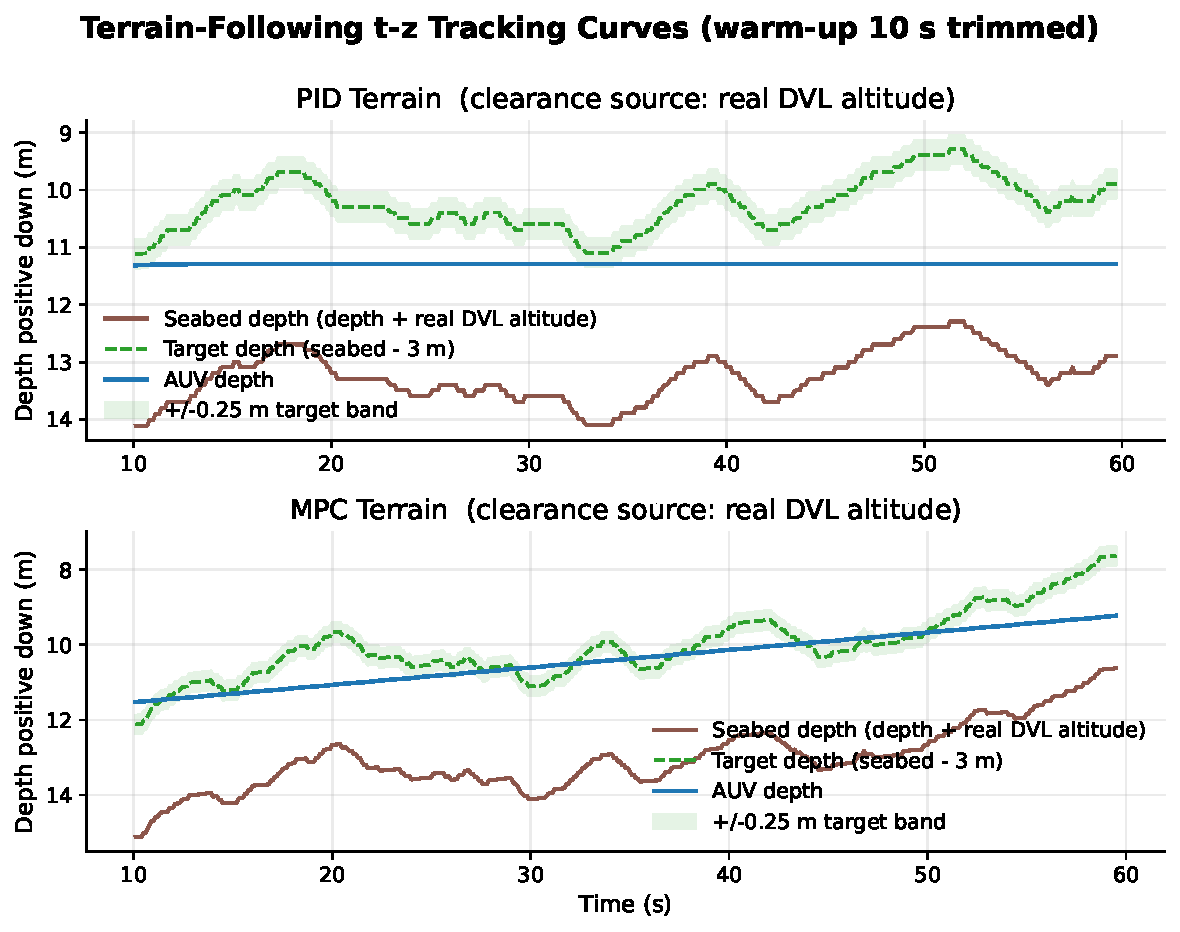
\includegraphics[width=0.95\linewidth,height=\textheight,keepaspectratio,alt={PID/MPC 地形跟随的分层深度响应：海底、几何目标、下发命令、PVS 可行参考与 AUV 真值深度}]{terrain_following/terrain_tz_tracking_pid_mpc.pdf}
\caption{PID/MPC 地形跟随的分层深度响应（原生 PVS 执行链，\(n=1\)）：两类制导均经同一 PVS 深度--航向内环}\label{fig:ch05-terrain-tracking}
\end{figure}
\FloatBarrier

图~\ref{fig:ch05-terrain-tracking} 从时间维度刻画了深度控制链，但难以直观呈现车辆如何在起伏海床上方保持净空。为补足空间直觉，图~\ref{fig:ch05-terrain-3d} 给出 PID 地形跟随相的三维真值轨迹。海底曲面由本次运行所用的确定性地形配置离线重建，其起伏公式与仿真地形生成逻辑同源（同一 seed 与噪声参数），因而覆盖 AUV 全程轨迹，而非使用 bag 中仅围绕原点的静态显示点云。图中蓝色轨迹与绿色 3~m 几何净空目标保持一致趋势，二者的局部间距体现安全过滤和内层动力学造成的跟踪偏差。沿程 DVL 实测海底作为独立验证锚点，与重建曲面的相关系数约 1.00、均值偏差约 0.00~m、均方根偏差约 0.03~m。旧图采用存在近常量平移偏置的滤波位姿，曾把该偏差放大到约 0.39~m；本图改用同一录包中的 PVS 真值轨迹后消除了这一坐标口径混杂。该三维视图仍为单次运行（\(n=1\)），只作空间直觉与地形一致性佐证；第~\ref{sec:ch05-5-5-3}节 的历史多种子消融验证高层地形与安全逻辑，不能替代当前原生 PVS 配置的重复试验。

\begin{figure}[htbp]
\centering
\includegraphics[width=0.9\linewidth,height=\textheight,keepaspectratio,alt={三维海底曲面与 PID 地形跟随真值轨迹：蓝色轨迹位于重建海床上方，绿色虚线为 3 m 几何净空目标，橙色散点为 DVL 实测海底验证锚}]{terrain_following/terrain_3d_pid_terrain_trajectory.pdf}
\caption{三维海底曲面与 PID 地形跟随真值轨迹（确定性地形重建 + 沿程 DVL 验证锚，\(n=1\)）：重建海床与 DVL 沿程海床的相关系数约 1.00、均方根偏差约 0.03~m}\label{fig:ch05-terrain-3d}
\end{figure}
\FloatBarrier

\subsection{PID 地形跟随的地形强度消融}\label{sec:ch05-5-5-3}

为验证地形参考与安全过滤层的多种子稳定性，本节对低、中、高三档地形强度各跑三个随机种子复验，并对其中两档落盘失败的种子各做一次重跑。该历史矩阵使用运动学设定点后端，故可支撑高层地形与安全逻辑的稳健性，但不能替代上一节调优后原生 PVS 深度内环的多次重复。最终合并口径如下（部分档的三种子由主跑成功种子与重跑成功种子合并得到，重跑原因是记录落盘不稳定而非算法闭环失败）：

\begin{longtable}[]{@{}
  >{\raggedright\arraybackslash}p{(\linewidth - 10\tabcolsep) * \real{0.1304}}
  >{\raggedleft\arraybackslash}p{(\linewidth - 10\tabcolsep) * \real{0.1739}}
  >{\raggedleft\arraybackslash}p{(\linewidth - 10\tabcolsep) * \real{0.1739}}
  >{\raggedleft\arraybackslash}p{(\linewidth - 10\tabcolsep) * \real{0.1739}}
  >{\raggedleft\arraybackslash}p{(\linewidth - 10\tabcolsep) * \real{0.1739}}
  >{\raggedleft\arraybackslash}p{(\linewidth - 10\tabcolsep) * \real{0.1739}}@{}}
\caption{PID 地形跟随三档多种子消融结果（运动学设定点后端）}\label{tab:ch05-terrain-ablation}\tabularnewline
\toprule\noalign{}
地形强度 & 成功/总数 & 离底 RMSE（m，均值±标准差） & 平均离底（m，均值±标准差） & 最小离底（m，均值±标准差） & \textless{} 1.5 m 违规 \\
\midrule\noalign{}
\endfirsthead
\toprule\noalign{}
地形强度 & 成功/总数 & 离底 RMSE（m，均值±标准差） & 平均离底（m，均值±标准差） & 最小离底（m，均值±标准差） & \textless{} 1.5 m 违规 \\
\midrule\noalign{}
\endhead
\bottomrule\noalign{}
\endlastfoot
低 & 3/3 & 0.587±0.112 & 3.546±0.146 & 3.259±0.388 & 0.0000 \\
中 & 3/3 & 0.709±0.002 & 3.709±0.002 & 3.708±0.002 & 0.0000 \\
高 & 3/3 & 0.610±0.081 & 3.583±0.112 & 3.228±0.205 & 0.0000 \\
\end{longtable}

三档地形均三次全部完成、无一例低于 1.5 m 的安全违规，离底 RMSE 落在 0.59--0.71 m 区间，说明地形参考与安全过滤在当前运动学后端和地形模型下具有稳定的近底安全性；该均值±标准差不外推为原生 PVS 内环的稳健统计。
三档消融的定量结论以表~\ref{tab:ch05-terrain-ablation} 为准，完整产物索引见附录。
\FloatBarrier

\subsection{MPC 极端平面路径支线结果}\label{sec:ch05-5-5-4}

本表为删除测试脚手架中一处常值下游偏置后的公平口径重跑结果：该偏置曾把整条 MPC 参考推向最近点下游、迫使 MPC 切弯并人为放大其横向误差，而两条 PID 基线不受影响，删除该偏置（保留真实预瞄项）后各变体一致复跑，样本量与适用边界见附录 A.7。下表为无扰动确定性单次运行（\(n=1\)），其后另附受控扰动的五种子（\(n=5\)）统计以支撑主结论。

本组实验把离线规划的长波与短波 S 弯、直角折弯与发卡掉头四类极端路径，分别交给仅调航向的 PID、视线制导（LOS）与 MPC 跟踪，比较横向跟踪误差。作为对照基线，LOS 的几何前视形式沿用经典制导方法\cite{breivik2005guidance,fossen2015los}，结果如下：

\begin{longtable}[]{@{}
  >{\raggedright\arraybackslash}p{(\linewidth - 8\tabcolsep) * \real{0.1667}}
  >{\raggedleft\arraybackslash}p{(\linewidth - 8\tabcolsep) * \real{0.2222}}
  >{\raggedleft\arraybackslash}p{(\linewidth - 8\tabcolsep) * \real{0.2222}}
  >{\raggedleft\arraybackslash}p{(\linewidth - 8\tabcolsep) * \real{0.2222}}
  >{\raggedright\arraybackslash}p{(\linewidth - 8\tabcolsep) * \real{0.1667}}@{}}
\caption{模型预测控制极端平面路径公平口径结果}\label{tab:ch05-mpc-extreme-paths}\tabularnewline
\toprule\noalign{}
场景 & 仅航向 PID 横向 RMSE（m） & LOS 横向 RMSE（m） & MPC 最优横向 RMSE（m） & 结论 \\
\midrule\noalign{}
\endfirsthead
\toprule\noalign{}
场景 & 仅航向 PID 横向 RMSE（m） & LOS 横向 RMSE（m） & MPC 最优横向 RMSE（m） & 结论 \\
\midrule\noalign{}
\endhead
\bottomrule\noalign{}
\endlastfoot
长波 S 弯（60 m / 7 m） & 0.093 & 1.047 & 0.055 & MPC 均优（较仅航向 −41\%、较 LOS −95\%） \\
发卡 180° 掉头 & 4.69 & 4.69 & 2.277 & MPC 均优（−51\%） \\
短波 S 弯 & 2.597 & 1.657 & 1.655 & MPC 较仅航向 −36\%、与 LOS 持平 \\
直角折弯 & 3.596 & 0.659 & 1.452 & 诚实边界：直角折弯上 LOS 前瞻最优 \\
\end{longtable}

\textbf{结论与边界}：公平口径下（同源 Bag、同一评价脚手架），MPC 在长波 S 弯、发卡掉头、短波 S 弯三类工况均优于或持平基线，长波 S 弯与发卡掉头上对两条基线均优于基线，短波 S 弯上优于仅航向 PID 且与 LOS 持平。唯一的诚实边界是直角折弯：该路径由分段直线组成，视线制导的几何前瞻最贴合，横向 RMSE（0.659 m）优于 MPC（1.452 m），此边界予以保留、不作过度宣称。早先``MPC 未普遍优于基线''的判断源自测试脚手架的偏置错误，修复后已被推翻。

为把上表的单次结论提升为可作主结论的统计证据，本文进一步在同一离线闭环中注入受控外部扰动（恒定横流不超过 0.15 m/s、初始横向偏移不超过 0.8 m、逐步艏向白噪声不超过 1.5°），以随机种子固定其实现，并令三种控制器在同一种子下共享同一扰动实现以保证公平；每类路径的 MPC 权重变体冻结为上表选定者，避免逐种子挑选。五个种子下横向 RMSE 的均值与标准差（单位 m）为：长波 S 弯，仅航向 PID $2.18\pm1.10$、LOS $1.15\pm0.15$、MPC $0.13\pm0.03$；发卡掉头，$4.50\pm1.28$、$4.25\pm0.46$、$2.36\pm0.23$；短波 S 弯，$2.73\pm0.31$、$1.67\pm0.04$、$1.82\pm0.19$；直角折弯，$3.43\pm0.46$、$1.00\pm0.51$、$1.57\pm0.46$。长波 S 弯与发卡掉头上 MPC 相对 LOS 的优势达到均值加减一倍标准差区间互不重叠的程度，短波 S 弯上 MPC 与 LOS 统计持平且均优于仅航向 PID，直角折弯上 LOS 仍最优。多种子统计因此支持上表的单次判断，MPC 制导层的多步预瞄与速度规划对复杂曲率路径具有可复现的横向误差优势，直角折弯的视线制导边界亦稳定成立。

长波 S 弯、短波 S 弯、发卡 180° 掉头与直角折弯的单次轨迹仅用于解释响应形态；多种子定量结论以表~\ref{tab:ch05-mpc-extreme-paths} 为准，完整轨迹产物与复现入口见附录。
\FloatBarrier

\subsection{不确定性感知控制主消融结果}\label{sec:ch05-5-5-6}\label{sec:ch05-5-5-7}

不确定性感知控制与固定权重基线的主消融在三个场景（基线、重度 DVL 丢包、综合压力）、两种控制模式、三个种子下执行，共十八次运行，全部成功（各行 3/3）且无安全违规。表~\ref{tab:ch05-uampc-control}并列给出定位侧（水平/深度 RMSE，来自离线滤波评估）与控制侧（横向 RMSE、控制变化率、安全违规率）的关键指标；圆概率误差与水平 RMSE 数值等价，不再单列，求解可解性与失败耗时采用具有完整诊断字段的可解性专项与最大迭代专项口径（见第~\ref{sec:ch05-5-5-8}节）。

\begingroup
\small
\setlength{\tabcolsep}{2pt}
\begin{longtable}[]{@{}
  >{\raggedright\arraybackslash}p{(\linewidth - 12\tabcolsep) * \real{0.12}}
  >{\raggedright\arraybackslash}p{(\linewidth - 12\tabcolsep) * \real{0.14}}
  >{\raggedleft\arraybackslash}p{(\linewidth - 12\tabcolsep) * \real{0.15}}
  >{\raggedleft\arraybackslash}p{(\linewidth - 12\tabcolsep) * \real{0.13}}
  >{\raggedleft\arraybackslash}p{(\linewidth - 12\tabcolsep) * \real{0.17}}
  >{\raggedleft\arraybackslash}p{(\linewidth - 12\tabcolsep) * \real{0.15}}
  >{\raggedleft\arraybackslash}p{(\linewidth - 12\tabcolsep) * \real{0.09}}@{}}
\caption{不确定性感知控制主消融结果（定位侧与控制侧并列）}\label{tab:ch05-uampc-control}\label{tab:ch05-uampc-localization}\tabularnewline
\toprule\noalign{}
场景 & 模式 & 水平 RMSE（m） & 深度 RMSE（m） & 横向 RMSE（m） & 控制变化率 & 违规 \\
\midrule\noalign{}
\endfirsthead
\toprule\noalign{}
场景 & 模式 & 水平 RMSE（m） & 深度 RMSE（m） & 横向 RMSE（m） & 控制变化率 & 违规 \\
\midrule\noalign{}
\endhead
\bottomrule\noalign{}
\endlastfoot
基线 & 固定权重 & 4.62±0.61 & 0.30±0.003 & 0.0038±0.0004 & 0.14±0.01 & 0 \\
基线 & 不确定性感知 & 4.40±1.01 & 0.30±0.004 & 0.0037±0.0003 & 0.44±0.27 & 0 \\
重度 DVL 丢包 & 固定权重 & 3.49±0.95 & 0.29±0.001 & 0.0033±0.0003 & 0.13±0.06 & 0 \\
重度 DVL 丢包 & 不确定性感知 & 3.55±0.50 & 0.30±0.006 & 0.0039±0.0013 & 0.19±0.22 & 0 \\
综合压力 & 固定权重 & 4.11±0.11 & 0.29±0.004 & 0.0035±0.0002 & 0.14±0.07 & 0 \\
综合压力 & 不确定性感知 & 3.68±0.50 & 0.29±0.002 & 0.0029±0.0004 & 0.030±0.004 & 0 \\
\end{longtable}
\endgroup

结果收敛到两条主结论。其一，\textbf{综合压力下不确定性感知控制形成一致增益}：水平 RMSE 由 4.11 降至 3.68~m（改善约 10.4\%），横向 RMSE 由 0.0035 降至 0.0029~m（改善约 15.8\%，与定位侧方向一致），控制变化率同时由 0.14 降至 0.030；基线场景亦有约 4.7\% 的轻微定位改善。其二，\textbf{重度 DVL 丢包下不再有优势}：水平 RMSE 反而变差约 1.9\%、横向 RMSE 由 0.0033 增至 0.0039~m，说明速度观测严重丢失、状态校正能力下降后，控制层权重调度不再形成增益。六组对照均无安全违规，但这只说明本批次未触及安全边界，不能替代极端场景压力测试；定位侧指标来自离线滤波评估，故``性能优于基线''的判断须结合横向误差、回退率与控制努力综合成立，而非由定位单项断言。

\subsection{不确定性感知控制的消融变体设计与机制归因}\label{sec:ch05-5-5-8}

为把整体性能变化归因到具体机制，本文设置四个变体：A0 为固定权重基线，A1 为完整 UA-MPC，A2 关闭低置信度下的 S 型控制代价降权，A3 保留完整机制但令置信度映射指数 \(\alpha=1\)。可解性专项对 A0、A2 和 A3 各执行三场景、三种子共二十七次运行；A1 采用最大迭代专项中迭代上限 100 的同场景、同种子层作为默认对照。事件加权结果见表~\ref{tab:ch05-uampc-p1-feasibility}。

\begin{longtable}[]{@{}cllr@{}}
\caption{可解性专项默认层的 UA-MPC 可解性归因}\label{tab:ch05-uampc-p1-feasibility}\tabularnewline
\toprule\noalign{}
变体 & 机制设置 & 运行数 & 回退率 \\
\midrule\noalign{}
\endfirsthead
\toprule\noalign{}
变体 & 机制设置 & 运行数 & 回退率 \\
\midrule\noalign{}
\endhead
\bottomrule\noalign{}
\endlastfoot
A0 & 固定权重 & 9 & 1.000 \\
A1 & 完整 UA-MPC & 9 & 0.699 \\
A2 & 关闭 S 型控制代价降权 & 9 & 1.000 \\
A3 & \(\alpha=1\) 的线性映射 & 9 & 0.335 \\
\end{longtable}

A0 与 A2 均为全程回退，而保留 S 型降权的 A1 和 A3 恢复了部分求解成功，说明低置信度下释放控制权威是可解性改善的必要机制。A3 的回退率低于 A1，表明更线性的跟踪权重映射能够进一步扩大可行域，但这一结果尚不足以决定默认参数，因为可解性降低不能以实时性或路径末端行为恶化为代价。

为检验高回退是否主要由迭代上限过紧造成，最大迭代专项在 A1 参数下仅改变内点法最大迭代次数，完成三场景、三种子共二十七次运行。表~\ref{tab:ch05-uampc-p2-maxiter}中的失败耗时只统计当前周期可观测的设定点回退，不使用保持上一输出时携带的陈旧耗时字段。

\begin{longtable}[]{@{}rrrrrr@{}}
\caption{最大迭代次数独立对照}\label{tab:ch05-uampc-p2-maxiter}\tabularnewline
\toprule\noalign{}
迭代上限 & 诊断帧 & 回退率 & 成功帧均值（ms） & 失败占用（ms） & 水平 RMSE（m） \\
\midrule\noalign{}
\endfirsthead
\toprule\noalign{}
迭代上限 & 诊断帧 & 回退率 & 成功帧均值（ms） & 失败占用（ms） & 水平 RMSE（m） \\
\midrule\noalign{}
\endhead
\bottomrule\noalign{}
\endlastfoot
100 & 1027 & 0.699 & 13.49 & 88.41 & 1.538 \\
200 & 1024 & 0.685 & 15.00 & 192.21 & 1.532 \\
400 & 761 & 0.594 & 17.04 & 372.20 & 1.552 \\
\end{longtable}

从 100 提高到 200 只使回退率下降 1.4 个百分点，综合压力场景甚至由 0.657 上升到 0.736；提高到 400 后仍有 59.4\% 回退，失败占用达到控制周期的 3.7 倍，诊断帧相对 100 档减少约 26\%。因此，迭代上限偏紧不是高回退的主因，默认值保持 100；后续可解性改进应转向初值连续性、约束残差与软约束机制。

可解性专项与最大迭代专项的参考路径接近直线，毫米级横向误差不适合承担精度归因。高机动专项因此在置信度 \(c=0.3\)、迭代上限 100 下，以确定性运动学模型补充长波 S 弯与 \(180^\circ\) 发卡路径，四个变体均无求解回退。结果见表~\ref{tab:ch05-uampc-h4-maneuver}。

\begin{longtable}[]{@{}lrrrr@{}}
\caption{横向机动的精度归因}\label{tab:ch05-uampc-h4-maneuver}\tabularnewline
\toprule\noalign{}
变体 & S 弯 RMSE（m） & 固定时长进度 & 发卡有效段 RMSE（m） & 发卡末端 RMSE（m） \\
\midrule\noalign{}
\endfirsthead
\toprule\noalign{}
变体 & S 弯 RMSE（m） & 固定时长进度 & 发卡有效段 RMSE（m） & 发卡末端 RMSE（m） \\
\midrule\noalign{}
\endhead
\bottomrule\noalign{}
\endlastfoot
A0 & 0.0852 & 76.5\% & 0.1015 & 7.480 \\
A1 & 0.0754 & 85.8\% & 0.1003 & 7.484 \\
A2 & 0.0852 & 76.5\% & 0.1019 & 7.480 \\
A3 & 0.0740 & 86.6\% & 0.0972 & 7.563 \\
\end{longtable}

在长波 S 弯中，A1 相对 A0 的横向 RMSE 改善 11.6\%，固定时长进度提高 9.3 个百分点；A2 几乎逐位退化回 A0，因而 S 型控制代价降权同样构成精度侧主贡献。A3 相对 A1 仅再改善约 1.9\%，且发卡末端 RMSE 略有增大，故保留默认 \(\alpha=1.5\)。发卡路径首次达到 99\% 进度前，四个变体的 RMSE 均约 0.10 m；全时段约 3.2 m 的大误差来自约 52 s 完成路径后车辆继续前进，属于终端停止条件缺失，而不是 \(180^\circ\) 转弯段跟踪失败。高机动专项用于隔离横向精度机制，不替代六自由度多种子或真机结论。

在上述机制归因之外，热启动与软约束实验进一步把运行期可解性拆为热启动与软约束两个独立因素。实验先统一预测时域、权重、约束和 20 Hz 调度周期，再在基线闭环中对四种组合各运行三个种子；按有效控制周期加权的结果见表~\ref{tab:ch05-r16-feasibility}。热启动硬约束配置同时取得最低回退率、最低周期阻塞率和最短平均求解时间；软约束只在少量失败周期中产生不超过 \(3.81\times10^{-3}\) 的松弛，却显著增加迭代数与求解时间，因而不能作为默认可解性修复。

\begin{longtable}[]{@{}ccrrrrr@{}}
\caption{热启动与软约束的三种子闭环对照}\label{tab:ch05-r16-feasibility}\tabularnewline
\toprule\noalign{}
热启动 & 软约束 & 有效周期 & 回退率 & 阻塞率 & 平均耗时（ms） & 平均迭代数 \\
\midrule\noalign{}
\endfirsthead
\toprule\noalign{}
热启动 & 软约束 & 有效周期 & 回退率 & 阻塞率 & 平均耗时（ms） & 平均迭代数 \\
\midrule\noalign{}
\endhead
\bottomrule\noalign{}
\endlastfoot
关闭 & 关闭 & 355 & 0.0169 & 0.0169 & 17.40 & 18.08 \\
关闭 & 开启 & 347 & 0.0375 & 0.1758 & 34.69 & 23.72 \\
开启 & 关闭 & 347 & 0.0086 & 0.0086 & 11.29 & 9.98 \\
开启 & 开启 & 343 & 0.0292 & 0.0437 & 30.32 & 21.50 \\
\end{longtable}

参考斜坡、软约束与终端保持的确定性消融则回答了另外两个问题。参考斜坡把发卡有效段 RMSE 从约 0.100 m 增至 0.424 m，不作为默认机制；终端保持不改变有效段精度，并把发卡末端 RMSE 从 7.484 m 降至 3.288 m，说明路径完成后应由任务层切换到终端状态。当前简化动力学不含反推力，零推进后仍存在被动漂移，因此该结果只支撑``终端任务定义有效''，不外推为定点保持精度。综合四组闭环统计与机制消融，本文冻结热启动开启、软约束关闭、迭代上限 100 的控制配置，并把终端保持作为独立任务状态。


\subsection{极端电缆巡检场景设计}\label{sec:ch05-5-7}

针对``场景真实性不足''这一问题，本节通过定义六个极端电缆巡检场景给出系统性补救方案。之所以需要单独设计一组极端场景、而不是简单把常规扰动幅度调大，原因在于极端工况的物理风险量级与常规消融不同，需要按几何极端、耦合极端、感知极端与多因素极端四类各自构造代表性场景，才能让``分层架构能否守住底线''这一问题获得有覆盖度的证据。六个场景按这一原则组织，各从路径设置、真实风险、观测角色与评价指标四个维度描述（见表~\ref{tab:ch05-extreme-scenarios}），并与第 4 章极端工况的``场景乘模式''二维消融设计相对应。

前两个场景检验几何极端：连续 S 弯是最先暴露预瞄能力差异的工况，视线制导在反向转弯过渡区因前视点跳变出现瞬态偏移，模型预测控制则因预测时域内能``看到''反向曲率而提前减小偏差；发卡掉头把转弯半径压到接近 AUV 的最小转弯半径，一旦几何不可行，即使最优预瞄也无法物理跟随，考察的是行为树能否触发``短时退出加重新对准''而不撞断电缆。陡坡穿越检验地形跟随与深度跟踪的协同，其难点在于水平推进与垂直深度调节必须在斜坡进入瞬间几乎同时完成，否则离底高度会短暂跌入 1.5~m 安全阈值以下。埋设间断检验声磁观测接力与滤波连续性：掩埋段内磁场特征突变、声呐几乎失去电缆边缘特征，AUV 须仅靠惯性递推与杆臂修正维持位置估计连续性，直至暴露段重新出现观测。横流冲击的扰动是持续而非瞬态的，欠驱动 AUV 没有横向执行器，只能通过航向偏置间接抵消，要求控制器在预测时域内识别横向偏移的累积趋势并主动给出航向偏置。综合极端场景把前五类因素叠加，用于同时压力测试``行为树高优先级子树是否按设计触发''、``控制器是否在多重压力下保持收敛''与``失联保护是否在极端通信扰动下兜底''三类问题，是判断分层架构能否在极端工况下守住安全底线（仿真）的最关键一项实验。

\begin{longtable}[]{@{}
  >{\raggedright\arraybackslash}p{(\linewidth - 10\tabcolsep) * \real{0.13}}
  >{\raggedright\arraybackslash}p{(\linewidth - 10\tabcolsep) * \real{0.27}}
  >{\raggedright\arraybackslash}p{(\linewidth - 10\tabcolsep) * \real{0.18}}
  >{\raggedright\arraybackslash}p{(\linewidth - 10\tabcolsep) * \real{0.22}}
  >{\raggedright\arraybackslash}p{(\linewidth - 10\tabcolsep) * \real{0.18}}@{}}
\caption{六类极端电缆巡检场景设定}\label{tab:ch05-extreme-scenarios}\tabularnewline
\toprule\noalign{}
场景 & 路径设置 & 真实风险 & 观测角色 & 评价指标 \\
\midrule\noalign{}
\endfirsthead
\toprule\noalign{}
场景 & 路径设置 & 真实风险 & 观测角色 & 评价指标 \\
\midrule\noalign{}
\endhead
\bottomrule\noalign{}
\endlastfoot
连续 S 弯急弯 & 两个反向圆弧，半径 15 m，总长 200 m & 舵角饱和导致跟踪失败 & 不确定性感知预瞄对视线制导预瞄 & 最大横向偏移、控制量平滑度 \\
发卡掉头 & 180° 掉头，半径 10 m & 最小转弯半径不足，路径不可行 & 预测时域能否提前预判 & 跟踪失败距离、航向误差 \\
陡坡穿越 & 电缆沿 30° 斜坡上升 5 m & 离底高度骤降，碰撞风险 & 两种地形跟随策略对比 & 最小离底高度、深度误差 \\
埋设间断 & 50 m 掩埋段 + 20 m 暴露段 + 50 m 掩埋段 & 磁场特征突变导致定位漂移 & 声磁接力切换 & 检测连续性、埋深反演误差 \\
横流冲击 & 直线电缆，横流 0.5 m/s & 横向偏移持续积累，舵角饱和 & 预测前馈对反馈补偿 & 稳态横向偏移、控制努力 \\
综合极端 & S 弯 + 发卡 + 陡坡 + 横流，叠加 DVL 丢包 30\% + 磁畸变 + 声呐杂波 & 多重失效耦合 & 系统整体鲁棒性 & 路由完成率、安全违规率 \\
\end{longtable}

六类场景的闭环统计和原生因子契约统一在下一节给出。

\subsubsection{代理正式矩阵、CBF 安全过滤与原生因子闭环}\label{sec:ch05-5-7-7}

六类代理电缆场景用于检验完整 ROS2 控制栈在``几何、地形、感知质量、横流''四类压力下的闭环行为。实验包括 6 个场景、固定权重与保守分源不确定性感知控制（下称 UA）两种模式、三个随机种子、每次 60 s，共 36 次运行。全部运行均完成并生成非空记录，运行契约完整，无失败事件；两种模式的求解回退均为 0，平均求解耗时 p95 分别约为 9.93 ms 和 9.82 ms。早期代理矩阵中的高回退现象在该同口径矩阵中未复现。

分源置信矩阵的主要性能结果见表~\ref{tab:ch05-r13-v2-main-results}。表中报告横向 RMSE、控制变化率、安全违规和授权模式四类结果。保守 UA 并未系统改善横向 RMSE；全局均值由固定权重的 7.932 m 变为 8.006 m。但它显著降低了多类高压力场景的控制变化率，全局 RMS 由 0.247 降为 0.085，其中发卡、横流和综合极端分别降低约 89.8\%、52.0\% 和 84.4\%。因此，该矩阵支持``分源置信下的保守控制平滑与实时可解性''，不支持``路径跟踪精度全面提升''。

\begin{longtable}[]{@{}
  >{\raggedright\arraybackslash}p{0.15\linewidth}
  >{\centering\arraybackslash}p{0.18\linewidth}
  >{\centering\arraybackslash}p{0.12\linewidth}
  >{\centering\arraybackslash}p{0.14\linewidth}
  >{\centering\arraybackslash}p{0.17\linewidth}
  >{\centering\arraybackslash}p{0.10\linewidth}@{}}
\caption{不确定性感知控制六类代理场景三种子正式结果}\label{tab:ch05-r13-v2-main-results}\tabularnewline
\toprule\noalign{}
场景 & RMSE 固定/UA（m） & RMSE 变化 & 控制变化率变化 & 安全违规固定/UA & UA 跟踪态占比 \\
\midrule\noalign{}
\endfirsthead
\toprule\noalign{}
场景 & RMSE 固定/UA（m） & RMSE 变化 & 控制变化率变化 & 安全违规固定/UA & UA 跟踪态占比 \\
\midrule\noalign{}
\endhead
\bottomrule\noalign{}
\endlastfoot
连续 S 弯 & 5.898 / 6.002 & +1.77\% & -24.50\% & 0.000 / 0.000 & 0.691 \\
发卡掉头 & 6.017 / 6.013 & -0.06\% & -89.79\% & 0.000 / 0.000 & 0.160 \\
坡面穿越 & 4.140 / 4.127 & -0.33\% & +15.95\% & 0.000 / 0.000 & 0.690 \\
埋设间断 & 4.136 / 4.053 & -2.01\% & +2.27\% & 0.000 / 0.000 & 0.542 \\
横流冲击 & 15.052 / 15.484 & +2.87\% & -52.02\% & 0.000 / 0.000 & 0.645 \\
综合极端 & 12.349 / 12.356 & +0.06\% & -84.40\% & 0.290 / 0.287 & 0.000 \\
\end{longtable}

分源置信链的核心证据来自授权模式和 \(p_{\mathrm{track}}\) 分布，而不是来自单一 RMSE 数字。声呐源提供 \(p_{\mathrm{track}}\)，磁源只提供检测概率；授权逻辑再按进入/退出阈值和去抖规则在保持、搜索与跟踪之间切换。六类场景的差异汇总于图~\ref{fig:ch05-r13-v2-evidence}：连续 S 弯、坡面和横流多处于跟踪态，发卡因有效观测稀疏而保持态增加，埋设间断同时跨越三类授权且逐次 \(p_{95}-p_5\) 均值约 0.483，综合极端则因未越过跟踪进入门而停留在搜索/保持边界。这说明授权机制没有把低质量观测误用为连续跟踪许可。

\begin{figure}[!t]
\centering
\subcaptionbox{保守 UA 对控制变化率的影响\label{fig:ch05-r13-v2-control-rate}}{%
  \includegraphics[width=0.72\linewidth,height=0.21\textheight,keepaspectratio,alt={六类代理场景中固定权重与保守不确定性感知控制的控制变化率成对对比；发卡、横流和综合极端显著下降}]{experiments/control/r13_v2_control_rate_paired.pdf}}\\[1pt]
\subcaptionbox{分源置信下的授权模式分布\label{fig:ch05-r13-v2-authority}}{%
  \includegraphics[width=0.72\linewidth,height=0.21\textheight,keepaspectratio,alt={保守不确定性感知控制下六类代理场景的保持、搜索、跟踪授权占比堆叠图}]{experiments/control/r13_v2_authority_modes_ua.pdf}}\\[1pt]
\subcaptionbox{分源置信 \(p_{\mathrm{track}}\) 分布\label{fig:ch05-r13-v2-ptrack}}{%
  \includegraphics[width=0.72\linewidth,height=0.21\textheight,keepaspectratio,alt={保守不确定性感知控制下六类代理场景声呐 p_track 分布箱线图；埋设间断动态范围最大，综合极端未达到跟踪进入门}]{experiments/control/r13_v2_p_track_boxplot_ua.pdf}}
\caption{不确定性感知控制的分源置信证据三面板：(a) 保守 UA 对控制变化率的影响；(b) 授权模式分布；(c) \(p_{\mathrm{track}}\) 分布}\label{fig:ch05-r13-v2-evidence}
\end{figure}

为了关闭速度门控的遥测缺口，本文在不改变 36 次正式矩阵结论的前提下补充遥测与授权审计。原矩阵 36 次运行均未记录策略后目标速度和控制器实际消费的授权快照，因此只能支撑控制平滑、回退与授权分布结论；补入请求/施加目标速度和授权快照后，四类场景共 12 次约 60 s UA-only 运行全部有效，速度与授权快照缺失均为 0。质量控制策略接受率均值为 0.995，速度缩放最小值、逐次 \(q_5\) 下界和均值分别为 0.000、0.805 和 0.896，最大施加速度动态范围 0.285 m/s，回退为 0，求解耗时 p95 上界 13.43 ms。该补强仅证明保守策略确实改变 MPC 消费目标速度，不替换表~\ref{tab:ch05-r13-v2-main-results} 的正式成对统计。

综合极端另以固定权重基线做三种子 60 s 全流程补充，结果见表~\ref{tab:ch05-r13-v16-combined-baseline}：3/3 完成，控制设定点全程处于巡缆跟踪状态，横向偏移 q50/q95 均值为 0.147/0.206 m，最大值 0.235 m，跟踪授权占比均值 0.982，回退与安全违规为 0。该组结果只作为搜索/保持边界之外的补充正证据，说明基础巡缆链路在最复杂代理场景下可重复闭合。

\begin{longtable}[]{@{}
  >{\raggedright\arraybackslash}p{0.18\linewidth}
  >{\centering\arraybackslash}p{0.09\linewidth}
  >{\centering\arraybackslash}p{0.14\linewidth}
  >{\centering\arraybackslash}p{0.14\linewidth}
  >{\centering\arraybackslash}p{0.11\linewidth}
  >{\centering\arraybackslash}p{0.12\linewidth}@{}}
\caption{综合极端固定权重全流程 60 s 三种子补充结果}\label{tab:ch05-r13-v16-combined-baseline}\tabularnewline
\toprule\noalign{}
运行口径 & 成功次数 & 横向偏移 q50（m） & 横向偏移 q95（m） & 跟踪占比 & 回退 / 安全违规 \\
\midrule\noalign{}
\endfirsthead
\toprule\noalign{}
运行口径 & 成功次数 & 横向偏移 q50（m） & 横向偏移 q95（m） & 跟踪占比 & 回退 / 安全违规 \\
\midrule\noalign{}
\endhead
\bottomrule\noalign{}
\endlastfoot
固定权重全流程, 60 s & 3/3 & 0.147 & 0.206 & 0.982 & 0 / 0 \\
\end{longtable}

近底安全方面，第~\ref{sec:ch04-4-4-7} 节定义的 CBF 过滤器在低、中、高三档地形和 PID/MPC 两类控制器下复核，共 18 个约 60 s 运行均有效。逐档结果见附录表~\ref{tab:ch05-cbf-terrain-matrix}：1.5 m 安全违规率和海床穿透率均为 0，最小净空下界为 2.70--2.90 m，18 个运行均触发速度门控，全局最低速度缩放为 0.180；MPC 9 个运行回退均为 0，求解耗时 p95 上界 23.84 ms。该矩阵支撑近底安全过滤有效，其代理口径与实时性边界连同本组其余不可外推项，一并归入下文``边界与负结果集中说明''。

\subsubsection{边界与负结果集中说明}\label{sec:ch05-r13-boundaries}

本组实验的负结果与不可外推项——代理场景横向 RMSE 未系统改善、综合极端未进入跟踪态、速度门控仅由补强证明、旧代理矩阵回退失败归因，以及 CBF 仍为手动设定点加运动学代理口径、其求解耗时 p95 上界不等于 10 ms 硬实时——的具体数字与机理归因，随第~\ref{sec:ch05-5-6}节 的证据边界总表统一给出。其中代理场景横向 RMSE 边界已由表~\ref{tab:ch05-r13-v2-main-results} 的成对 RMSE 与变化率列直接读出。

为避免继续用配置拼装代替场景物理契约，本文另建立原生因子生成器。电缆中心线由分段几何和随地形变化的埋深共同定义，磁真值由同一中心线的分段 Biot--Savart 积分生成，声呐可见性由埋深决定，横流独立作用于水体速度；实测三轴噪声只进入量测副本，不能修改电缆、地形、磁场或流场真值。曲线几何、地形与埋设、实测噪声回放、横流四个因子各自独立开关，\(2^4\) 个组合各取两个种子，共 32 次契约验证全部有效。

\begin{longtable}[]{@{}llll@{}}
\caption{原生场景因子开关验证}\label{tab:ch05-r21-native-factors}\tabularnewline
\toprule\noalign{}
因子 & 关闭口径 & 开启口径 & 可观测差异 \\
\midrule\noalign{}
\endfirsthead
\toprule\noalign{}
因子 & 关闭口径 & 开启口径 & 可观测差异 \\
\midrule\noalign{}
\endhead
\bottomrule\noalign{}
\endlastfoot
电缆几何 & 直线 & 分段曲线 & 中心线真值独立改变 \\
地形与埋设 & 平底、0.15 m & 起伏地形、最大 1.40 m & 声呐可见率 1.000 降至 0.845 \\
磁噪声 & 同协方差高斯 & 实测三轴循环回放 & lag-1 相关 \(-0.024\) 变为 \(-0.998\) \\
横流 & 0 m/s & 时变横流 & 平均流速 0.352 m/s \\
\end{longtable}

原生场景因子实验闭合的是``因子可独立操纵、真值与量测不串扰''这一生成器契约，而非控制性能结论；表中给出四个因子开关的可观测差异，噪声时间结构与横流时序的完整产物索引见附录。原生因子闭环实验在此基础上把原生生成器接入制导级 MPC、分源跟踪授权和保守质量控制策略，形成不调用 PVS 原生定深定向自驾的全因子离线闭环矩阵，用于排除原生声磁、地形与横流因子无法进入控制闭环的接口风险，并量化主效应与二阶交互。

原生因子闭环全矩阵覆盖曲线几何、地形/埋设、实测磁噪声回放与横流四个因子的 \(2^4\) 个组合，每组 3 个种子，并分别运行固定权重基线与保守不确定性感知控制，共 96 次、每次 20 s。全部运行有效，回退、1.5 m 低净空违规和海床穿透均为 0；最坏横向 p95 为 1.716 m，最小净空为 2.536 m。求解耗时 p95/max 上界为 24.02/38.83 ms，相对 20 Hz ROS 控制、10 Hz 桥接/主控和约 0.3 s 网络接收预算均未越界，全矩阵与时序审计见附录表~\ref{tab:ch05-r22-native-factorial}。

因子效应上，横流是横向 p95 的主导因子，跨模式主效应约 0.639 m；曲线几何与横流构成主要二阶交互，跨模式约 0.396 m。地形/埋设与实测噪声回放在 20 s 短时窗口内主效应接近零，说明当前压力主要来自平面几何和水体速度。不确定性感知控制的收益仍应按控制风格表述：平均控制变化率 RMS 从约 4.831 降至约 0.814，但平均横向 p95 从约 1.173 m 增至约 1.206 m；困难的曲线加横流组合中最坏 p95 由 1.716 m 降至约 1.625 m，只能写成边界样本上的平滑收益。

为检查短时窗口是否掩盖误差累积，本文随后运行三组仿真侧补强。60 s 全 \(2^4\) 矩阵共 96 次运行，全部有效且回退、安全违规和穿底均为 0，最坏横向 p95 为 2.176 m，最小净空 2.384 m；终端审计显示 96 次均未触发有限参考路径末端，因此全窗口指标可视作活动巡缆段指标。120 s 地形加横流固定时长边界矩阵共 24 次运行，安全违规仍为 0，但全窗口最坏横向 p95 达到 6.839 m；分段审计发现 24/24 次均在 65.0--105.0 s 到达路径终点，活动段横向 p95 最大 2.152 m、终端尾段最大 7.703 m。加入任务层到达即退出后，同一专项 24/24 到达并退出，最坏横向 p95 回落到 2.152 m，说明固定时长恶化来自路径完成后的终端尾段，而非主矩阵接口结论被推翻。该归因指向的是到达终点后的漂移尾段，而非定点保持或横流悬停能力。

为关闭离线仿真代理尚未覆盖的执行链风险，本文另运行一次 PVS 原生定深定向冒烟实验。专用配置将 PVS 控制模式置为定深定向自驾、运动模型置为原生，ROS2 控制器、MPC 与仲裁器经二进制下行进入模拟管理设备自动分发后触发 PVS 内层自驾。审计显示自动模式命中 149 次、原生自驾后端开启 1 次、运动学代理日志为 0；记录到设定点 245 帧、控制命令 720 帧、滤波状态 998 帧，72 个控制器诊断样本均求解成功，耗时 p95/max 为 19.32/20.40 ms。该结果只支撑``PVS 原生仿真执行链已闭合''，尚不构成定深定向控制精度结论。

真机侧时序口径由 PC104 UDP 探针补充：同一 300 s 主机中继记录下，下行零推力包解析无误、上行帧号无前向缺口，应用路径 RTT 与固件内部时差的完整统计见第~\ref{sec:ch05-5-3-1}节。该 RTT 包含容器、宿主机中继、双向网络和固件周期调度，不构成任一方向的单向物理延迟。

\section{端到端数字孪生与闭环恢复}\label{sec:ch05-e2e}

第三条主线把前两条主线的估计与控制能力合拢为一条完整的海缆巡检任务，在高保真数字孪生后端上端到端运行，并给出两级证据：其一是干净先验下符合行业标准风格的数字孪生验收，其二是先验带偏差时的分层证据——从算法同源性、失效边界到满足磁观测前提的六自由度闭环恢复。二者共同界定端到端链路``已闭环到什么程度、在什么先验条件下成立''。

\subsection{海缆巡检的行业标准数字孪生验收结果}\label{sec:ch05-5-5-10}

前面几节从控制侧压力测试考察闭环可运行性，本节报告一条独立、保真度更高的证据链：在数字孪生后端上运行完整海缆巡检任务，将电缆跟踪结果记录后进行离线评分，并形成参照《DL/T 1278---2025 海底电力电缆运行规程》\cite{dlt1278_2025}的评价结果。评分链路、阈值定义与处理参数见附录 A.8。三次相互独立的实时运行构成多次运行聚合结论。

一组约 120 s 的初步运行用于检查``磁力计—跟踪—控制—记录—离线评分''工程链路及产物格式。该运行的跟踪置信度固定为 0.5，最大路由偏移约 14.7 m，且缺少埋深不确定度，因而只构成链路连通性证据，不进入验收结论。多次运行聚合仅采用引入质量与验收判定层后的三次独立运行，完整产物索引见附录 A.8。

三次全新运行的结果高度一致：原始样本约 1230--1250、有效样本约 770--790、就绪且通过工业验收，行业标准风格评分完全一致（总分 24、最差项 16、注意状态），扣分项均为``海缆埋深不足''与``埋深估计精度未达 0.15 m''两项。三次运行的排除样本构成一致，均为``离开 50 m 巡检窗口''、``埋深预热未就绪''与``越出路由走廊''三类，说明窗口化剔除的是末段到达终点后的漂移与起步预热，而非``裁剪到通过''。对三次运行聚合，通过率为三分之三、就绪分布一致，满足``至少三次运行且通过率不低于 0.67''的口径，因此初步验收就绪判定为真。这里的``初步''是刻意保留的限定词：它表示``在数字孪生证据链上，多次运行的证据完整性、起点健康、窗口有效性与工程阈值均一致通过''，而非``通过现场海试验收''。（三次运行的验收判据与聚合口径见附录 A.8。）

行业标准风格评分卡以图~\ref{fig:ch05-dlt-scorecard-run1} 为代表；三次运行评分一致，因而不重复展示第 2、3 次评分卡。电缆平面图、巡检窗口时间线、埋深不确定度诊断及界面回放等辅助产物不作为独立证据重复计数，其索引见附录 A.8。

\begin{figure}[htbp]
\centering
\includegraphics[width=0.95\linewidth,height=\textheight,keepaspectratio,alt={DL/T 1278 风格评分卡·第 1 次运行（数字孪生确定性先验；总分 24、最差项 16、注意状态，扣分为埋深不足与埋深精度未达 0.15 m；三次运行评分一致）}]{cable_acceptance/cable_dlt1278_scorecard_fresh1.pdf}
\caption{DL/T 1278 风格评分卡（数字孪生确定性先验；总分 24、最差项 16、注意状态，扣分为埋深不足与埋深精度未达 0.15 m；三次运行评分一致）}\label{fig:ch05-dlt-scorecard-run1}
\end{figure}
\FloatBarrier

上位机操作员工作流演示使用第一次运行的遥测逐帧驱动真实界面，在离屏模式下仅执行安全操作并停用外发定时器。该演示用于验证人机界面的数据契约，不计作新的算法证据；视频与末帧索引见附录 A.8。

\textbf{证据边界}：本节验收链路的口径限制已并入第~\ref{sec:ch05-5-6}节 的证据边界总表。近零路由偏移与近常值置信度只证明链路与评分逻辑正确，尚不能代表真实检测精度；就绪判定限定于有效巡检窗口，三次运行也是同一场景的连续重复。因此，本节结论限定为数字孪生确定性先验下的全链路就绪与初步验收，不等同于真实海缆检测精度或现场行业标准验收。

\subsection{先验偏差与六自由度闭环恢复}\label{sec:ch05-5-5-11}

主仓运行节点直接消费专用磁探测仓库的同源部署接口。干净先验与真实电缆重合时，评分链可通过，但这不足以证明初始误差下的捕获能力。算法级单次扫描表明，在线先验修正和自适应横切是关闭即失败机制；地图投影连续与车辆相对真缆的物理配准是不同指标。调优后 1.0/1.5/2.0 m 埋深的单周期 MAE 为 0.124/0.079/0.123 m，只是同源模型下的 $n=1$ 结果；后续 v2 用独立稳定性与模型失配实验进一步界定其适用范围。

先验带偏差时，分别运行中、重档各三次开环回放和六自由度闭环。在线修正未能接受观测的初始配置中，开环最大路由偏移分别约 15.4/20.3 m，闭环为 15.3/20.1 m，验收窗口内点数均为零。闭环确有操舵变化，因此失败不能归因于只回放固定轨迹。根因是产磁电缆与传感器近共面，违反直线埋缆分量比反演的几何前提；约 1200 帧观测被残差门拒绝。

将直缆布置在传感器下方约 7.5 m 后，解耦轻量闭环先确认修正接口接受观测，再迁回六自由度闭环。中、重档各三次约 98\% 观测被接受；重档起始横偏约 $-10.25$ m，约 12 s 内进入 $\pm3.4$ m 走廊。关闭在线修正的同源基线全部无效；开启后的六次均在规定窗口就绪并通过。图~\ref{fig:ch05-pvs-closedloop-recovery}给出物理配准与接受时序，表~\ref{tab:ch05-closed-loop-acceptance}列出最终窗口结果。

\begin{figure}[htbp]
\centering
\includegraphics[width=0.95\linewidth,height=\textheight,keepaspectratio,alt={六自由度闭环先验畸变恢复与在线先验修正接受时序（数字孪生确定性先验、静态位姿扭曲、缆在车下满足磁观测前提、窗口内判定，中/重档各 \(n=3\)）}]{cable_acceptance/pvs_closedloop_recovery_prior_alignment.pdf}
\caption{六自由度闭环先验畸变恢复与在线先验修正接受时序（数字孪生确定性先验、静态位姿扭曲、缆在车下满足磁观测前提、窗口内判定，中/重档各 \(n=3\)）}\label{fig:ch05-pvs-closedloop-recovery}
\end{figure}

\begin{table}[htbp]
\centering
\caption{六自由度闭环在线修正后的窗口内结果}\label{tab:ch05-closed-loop-acceptance}
\begin{tabular}{@{}lrrrr@{}}
\toprule
档位 & 通过次数 & 有效点数 & 最大横偏（m） & 平均横偏（m）\\
\midrule
中档 & 3/3 & 328--1029 & 3.395 & 2.412\\
重档 & 3/3 & 320--725 & 3.394 & 2.318\\
\bottomrule
\end{tabular}
\end{table}

两档有效埋深比均为 1、不确定度超限比为零、置信 5 分位最低为 0.902；最大与平均横偏分别按每档三次最差值报告，对应门限 3.4/2.5 m。恢复依赖满足观测几何、航向接口修正、0.6 m 扫描摆幅与 10 m 深度物理上限，不代表任意不利几何下自动恢复可观测性。该组仍是静态先验畸变、无真实检测噪声与硬件时延的数字孪生窗口证据，完整评价条件见附录~\ref{sec:app-a-9}。
\FloatBarrier

\subsection{显式 FWHM 的稳定性与场形适用边界}\label{sec:ch05-fwhm-stability}

独立 v2 模块补齐先验引导搜索、磁异常检测、主动横切、显式 FWHM 与沿缆跟踪。Cases A--D 分别覆盖大初始位置误差、埋深、噪声和搜索间距：20 种子基线中大初误差与各间距组均检测成功，无源虚警率为零，埋深组与噪声组 MAE 分别为 0.013/0.049 m。这些同源前向模型结果用于算法回归，不代表真实海缆精度。

50 种子设计消融将收益归结为四项可解释机制：扣背景半峰将距离 MAE 从 1.220 m 降至 0.010 m；以导航空间坐标替代均速乘时间，将非匀速扫描 MAE 从 0.855 m 降至 0.014 m；覆盖三倍垂距的自适应扫描有效率为 1.00，固定 1.5 m 扫描为零；三次扫描中值将单次离群下的宽度 MAE 从 0.466 m 降至 0.091 m。分段横切与正弦半周期均有效，前者 MAE 为 0.015 m，后者为 0.021 m。因此采用空间采样、逐级扩幅和重复确认，摆幅同时受沿缆漂移、载体机动与走廊约束。

为进一步区分``标称精度''与``扰动下仍可安全发布''，本文对显式空间 FWHM、自由幅值剖面拟合、标定幅值反演和未扣背景半高四种方法做稳定性对照。实验覆盖标称、增益变化、背景变化、噪声、扫描偏心、组合扰动和场模型失配七类场景，每类每种方法使用 200 个固定随机种子，共形成 5600 次方法运行。自由拟合同时估计背景、幅值、中心和尺度；幅值反演使用名义源强标定，并在背景实验中获得真实标量背景，因而是有利对照；FWHM 使用当时的双侧交点与几何质量门。本组结果作为新增场形判别门之前的冻结基线保留，不以修复后的结果覆盖。图~\ref{fig:ch05-fwhm-v2-stability} 给出条件精度、有效发布率、大误差发布风险和组合扰动误差分布。

\begin{figure}[htbp]
\centering
\includegraphics[width=0.96\linewidth,height=0.72\textheight,keepaspectratio,alt={显式空间 FWHM、自由幅值剖面拟合、标定幅值反演和未扣背景半高在独立扰动、组合扰动与场模型失配下的稳定性比较}]{experiments/fwhm_v2/11_fwhm_stability_comparison.pdf}
\caption{FWHM 与对照方法的稳定性比较（每场景每方法 200 个固定种子）}\label{fig:ch05-fwhm-v2-stability}
\end{figure}

组合扰动同时包含增益、背景、噪声和扫描偏心。显式 FWHM 的有效发布率、发布结果平均绝对误差、90\% 分位误差和误差超过 0.5 m 的发布比例分别为 0.970、0.105 m、0.235 m 和 0.055；自由幅值拟合对应为 1.000、0.171 m、0.433 m 和 0.085；标定幅值反演对应为 1.000、0.678 m、1.280 m 和 0.610。扫描偏心单项中，FWHM 只发布 74\% 的剖面，但已发布结果的 90\% 分位误差为 0.045 m，且没有大于 0.5 m 的发布，说明有效率下降来自对不完整双侧覆盖的选择性拒绝。增益变化单项中，FWHM 与标定幅值反演的平均绝对误差分别为 0.027 m 和 0.772 m，进一步说明宽度量对未知整体增益更稳定。关键扰动的连续敏感度见图~\ref{fig:ch05-fwhm-v2-sensitivity}。

\begin{figure}[htbp]
\centering
\includegraphics[width=0.96\linewidth,height=0.48\textheight,keepaspectratio,alt={FWHM、自由幅值剖面拟合和标定幅值反演对未知增益、测量噪声与场形模型失配的连续敏感度}]{experiments/fwhm_v2/12_fwhm_stability_sensitivity.pdf}
\caption{FWHM 与对照方法对增益、噪声和场形模型的敏感度}\label{fig:ch05-fwhm-v2-sensitivity}
\end{figure}
\FloatBarrier

该比较同时给出 FWHM 的适用边界：当前向场形由声明的偶极包络改为单直导线、反演仍沿用偶极场形系数时，FWHM 的平均绝对误差升至 2.753 m，且全部结果的误差均超过 0.5 m；自由拟合也出现 1.483 m 的系统误差。幅值反演在该特定失配中误差较小，是因为实验保留了相同峰值标定，并不意味着其一般优于宽度反演。因此本文的结论不是``FWHM 与模型无关''，而是``在场形模型已标定且扫描剖面完整时，FWHM 对整体增益和组合扰动更稳定''。工程上应在部署前用已知距离横切标定场形系数，并以模型身份或拟合残差阻止错误模型下的高置信度发布。

针对上述高置信度误发布风险，v2 在原质量门之后新增显式场形判别门：固定实测峰值、中心、半高宽和背景，在相同自由度下计算声明模型与备选模型的归一化剖面残差。只有备选模型残差比声明模型至少低 0.02，且不超过其 0.75 倍，才判为``备选场形明显更优''；此外要求峰值左右各有至少 0.65 个半高宽的空间支持。不满足时保留宽度和诊断量，但不发布垂向距离及埋深。阈值探索使用种子 0--199，留出验证独立使用 200--399。图~\ref{fig:ch05-fwhm-v2-shape-guard} 展示双向失配的拒绝效果及正确模型发布率代价。

\begin{figure}[htbp]
\centering
\includegraphics[width=0.96\linewidth,height=0.70\textheight,keepaspectratio,alt={留出种子验证形状判别门在偶极与单直导线双向失配中的大误差拒绝率、正确模型发布率和归一化残差散点}]{experiments/fwhm_v2/13_shape_guard_held_out_validation.pdf}
\caption{跨场形模型失配的识别与拒绝：独立留出种子验证}\label{fig:ch05-fwhm-v2-shape-guard}
\end{figure}
\FloatBarrier

留出集每场景 200 次。真实单直导线误声明为偶极，以及真实偶极误声明为单直导线时，旧门均在全部 200 次发布大于 0.5 m 的误差，新门在两组共 400 次均拒绝发布。正确声明的直导线、标称偶极、增益变化和背景变化各组仍全部有效；噪声组由 1.000 降至 0.990，出现两次误拒。扫描偏心的有效率由 0.740 降至 0.645，组合扰动由 0.925 降至 0.875，主要代价是外侧数据不足时保守拒绝；组合扰动中大于 0.5 m 的误差仍发布比例均为 0.030，故该门解决的是本实验两类场形混淆，不是全部大误差。单条剖面不能自行发现``场形正确但宽度到距离系数标错''；PVS 中点电流元和真实多芯铠装海缆也未纳入这次两模型留出验证，仍需已知距离的独立标定与受控实测。

为处理系数错误这一剩余风险，另实现受控横切标定与独立留出审计：训练扫描以已知传感器--导线垂距与实测半高宽的比值中位数估计场形系数，留出扫描再检查有效率、平均绝对误差及 95\% 分位误差；不合格则拒绝作为发布系数。解析式生成的各 50 条训练与 50 条留出扫描中，匹配单直导线和偶极包络分别取得 0.011 m 与 0.009 m 的留出平均绝对误差；将直导线留出剖面的表观宽度放大 50\% 而保持归一化形状不变，留出误差升至 1.809 m，标定被拒绝。这只证明软件流程能利用\emph{独立几何真值}发现形状门不可识别的系数漂移，不代表真实海缆精度。保守的多模型接口亦要求候选场形有通过实测留出的系数：模型不可区分或估计距离不一致时不发布埋深。当前仓库尚无满足导线位置、同步横切位姿及高度真值条件的实测标定集，因此不将该接口标记为实物部署已闭环。巡检 ROS 节点在非仿真时钟下还拒绝将未标定埋深发布开关置为真；这一入口门只防止配置误开启，不能替代实测标定及其接线。

进一步的跨场型探索说明仅比较偶极与单直导线仍不充分。100 种子留出中，真实幂律指数为 0.7 而沿用偶极固定系数时，全部扫描仍发布大于 0.5 m 的距离误差，发布结果平均绝对误差为 0.928 m；在预先限定的连续幂律家族内拟合指数，可把该误差降至 0.034 m。不过，近距双导线仍可能被单场形近似并发布。仓库既有有限线段场模型的归一化剖面近似偶极，宽度--距离系数却从 2 m 时的 0.433 变至 8 m 时的 0.495；在预定训练距离 2、4、8 m 和留出距离 3、6 m 上，受控仿射宽度标定将留出平均绝对误差从常系数的 0.121 m 降至 0.022 m。这些均为模型剖面或解析式数据，只论证\emph{限定场形家族内的估计改进与已知距离标定的必要性}；未知多芯海缆的真实埋深仍不可由单条磁剖面保证。


\subsection{横向定位与埋深的独立许可}\label{sec:ch05-inspection-contract}

对称单源剖面中，左右半高交点中点提供横向中心，宽度转为垂距仍需已知场形系数（第~\ref{sec:ch03-3-3-3}节）。v2 将横向定位、目标身份、埋深发布和自治执行分别授权：剖面不完整则有界重扫；缺合格场形标定或同步离底高度则埋深为空；身份、导航或控制来源失鲜则 Hold。单一高置信磁峰不证明目标身份，近邻源融合时须用独立目标锚点与全程排他走廊核验。声呐区间须完整落入目标走廊，不能只与锚点相交；无法排除邻缆时保留磁异常而拒绝跟踪。

真实测量的适用性由 TMR--ArUco 记录只读复核：777 个同步点可拆为九条单调扫描腿，四条通过运动质量门，但九条均缺少至少一个半高交点，允许发布深度的腿数为零。这验证了真实数据下的拒绝路径；自由手持记录缺少受控平面双侧横切和海床高度，不能改写成埋深标定集。

\subsection{限定条件下的磁巡检闭环结果}\label{sec:ch05-current-magnetic-closure}

当前源码、既有 PID、72 字节协议编解码与原生 PVS 在已知孤立直线磁源、理想导航、零横流和 6 m 先验横偏下复核。浅角扫描从 $(-250,-15)$ m 至 $(-80,15)$ m，前向接入为 20 m，航速 0.3 m/s；两种标量包络峰值 20 nT、背景 1 nT、垂向尺度 3 m，独立高斯噪声标准差 0.03 nT。名义 80 m 任务两端各留 5 m 缓冲，核验核心为 $[5,75]$ m。单直导线与偶极包络各三个噪声种子均完成并覆盖核心段，三个无源对照均拒绝 Track；埋深保持空值，九次无异常退出或非有限状态。

核心段内全部 Track 样本计入评价，包含回归修正：真实横偏 MAE 为 0.771--0.774 m、最大 1.321 m，满足预设平均不超过 1 m、最大不超过 2 m 的门。图~\ref{fig:ch05-current-magnetic-simulation-closure}展示巡检过程、磁中心估计与完整沿程误差。结果证明声明条件下的有限横向巡检可达；固定二维包络和理想导航尚不覆盖高度/姿态耦合、ROS 实时调度或实物输入。

\begin{figure}[htbp]
\centering
\includegraphics[width=0.96\linewidth,height=0.52\textheight,keepaspectratio,alt={当前磁巡检源码在限定条件下的搜索、主动横切、前向接入和有限跟踪；两场形中心估计与六条航迹的真实横向误差，含核心段全部回归修正}]{experiments/fwhm_v2/71_current_magnetic_simulation_closure.pdf}
\caption{当前磁巡检算法的限定条件仿真复核。阴影为 $70~\mathrm{m}$ 核验段，两端缓冲不计为核心覆盖；全部核心 Track 样本计入误差，埋深保持独立空值。地图横纵轴比例不同。}
\label{fig:ch05-current-magnetic-simulation-closure}
\end{figure}

\subsection{扰流、导航与多源的条件性监督}\label{sec:ch05-inspection-ros-boundary}\label{sec:ch05-inspection-robustness}

独立监督以报告位移与世界系地速的增量／有限窗一致性诊断导航跳变和漂移，并冻结完整横切剖面监测磁幅变化。仅当测得反向扰动代理超过 0.02 m/s 时，接入由 20 m 缩短为 5 m；该代理含侧滑，不等于直接流速测量。指定目标授权额外使用区间 $y=6\pm0.05$ m，假设水平导航硬误差不超过 0.10 m，以三角不等式预算核心横偏。外部参考不是磁算法独立识别的证据；无参考仅记录磁异常路线，不授权目标完成。

冻结参数后，20 条件、三个种子与两方法形成 120 次原生 PVS 留出。单源和未知对称包络、正反 0.03 m/s 稳态流、$\pm0.02$ m/s 周期流、小导航扰动、弱邻源及组合扰动共九类正例完成 27/27 次；全核心真实横偏 MAE 0.426--0.816 m、最大 0.775--1.552 m。其余十一类对照 33/33 撤权，错误几何授权与错误任务完成均为 0/60；旧链有 12/60 次错误几何授权，尽管融合邻源的载体误差可通过路线门（图~\ref{fig:ch05-inspection-robustness-summary}）。拒绝不算完成，截短误差不排名，有限网格不外推海况概率；未知场形的横向通过不授权埋深。

\begin{figure}[htbp]
\centering
\includegraphics[width=0.96\linewidth,height=0.38\textheight,keepaspectratio,alt={独立留出反向小流在条件式五米接入下完成真实核心段，旧二十米接入未覆盖；融合邻源的车辆误差通过相应门限但中心错误，额外参考监督拒绝目标授权}]{experiments/fwhm_v2/77_defense_robustness_thesis_summary.pdf}
\caption{条件式接入与目标几何授权的留出对照（额外外部参考）。左图含全部核心 Track，灰区为旧链未覆盖；右图按相应门限归一化。接入收益另经三次几何消融复核。}\label{fig:ch05-inspection-robustness-summary}
\end{figure}

无外部参考的九次消融均不授权指定目标；只改接入的反向小流三次合格完成，分离了几何与参考贡献。跳变同周期撤权，漂移用有限窗诊断；反向阶跃和超界流仍拒绝。监督撤权后 60 s 持续零命令，30 s 请求上级恢复但未模拟其实施，车辆仍滑行／漂移。保证只在参考和水平导航误差界实际成立时有效；共同偏差、曲线及完整三维多源场仍在范围外。

历史同版 ROS--PID--守卫--本地 UDP--原生 PVS 的八条有限航迹为七条到端、一条反向阶跃暂停；暂停后 241/241 周期零命令，60 s 仍移动 5.683 m。稳态最大横偏 0.742--1.234 m 相对估计线，不能替代本次相对真缆的误差；历史软件链与新增独立回路不拼为一次实时或实艇验收。

较宽先验采用连续余弦浅角多横切，每站形成空间磁剖面后联合估计线位和方向。扫描幅度、半波长与出口侧必须同时满足双侧覆盖、转弯能力、边界余量和后续接入预算。根据横流上游起始侧及目标侧选择三／四段，避免扫描有效却无法有限距离接入。独立 ROS 扩展在目标线 $y=5.5+0.02x$、合成横流 $\pm0.04$ m/s 下，正向三段与反向四段各三个噪声种子均完成 80 m Track，全部 Track 真值横偏 MAE 分别为 0.334--0.339 m 与 0.291--0.293 m；无源和融合邻源对照拒绝，身份失鲜后零命令仍伴随约 2.81 m/15 s 的滑行（图~\ref{fig:ch05-inspection-shallow-survey-ros}）。首个正向案例经过守卫与 UDP，追加种子仅经过 ROS/PID/协议/PVS，不能混作同一全栈样本量。

\begin{figure}[htbp]
\centering
\includegraphics[width=0.96\linewidth,height=0.63\textheight,keepaspectratio,alt={ROS多横切在正反横流下完成三段与四段扫描、接入和八十米跟踪，融合邻源和身份失鲜拒绝后原生PVS仍滑行}]{experiments/fwhm_v2/51_shallow_survey_ros_pvs_chain.pdf}
\caption{连续多横切接入 ROS 巡检链后的轨迹、横偏与分层拒绝（合成身份和横流）}\label{fig:ch05-inspection-shallow-survey-ros}
\end{figure}

上述多横切输入的身份与流速均为合成消息，三／四段解析覆盖余量仅 0.099/0.366 m，故保留为受限扩展结果。未知多源场形、严重横流低报和任意海况仍可能使接入或跟踪拒绝。扩大之字形幅度须有可执行走廊与观测收益支撑，不能仅为提高 FWHM 有效率而无条件增幅。
\FloatBarrier

\subsection{相对磁几何与海床基准的离线分项验证}\label{sec:ch05-round2-relative-reference}

2026年10月20日的独立离线补充将第~\ref{sec:ch02-2-3-5}节的条件几何进一步拆为横向坐标$c$、参考探头相对垂距$z_*$和轴深$d_{\mathrm{axis}}$。该原型不接入默认ROS巡检工厂，不替代前述70 m横向巡检、真实TMR或执行脑子链证据。磁输入只含实际生成的峰值复三轴观测与相对轨迹，绝对探头高度由另一独立参考提供；仿真真实深度及误差仅供评测。

已知平行三芯中心分布半径取0.15 m，合成外半径0.20 m；前者不是单个导体半径。A相实数残余比例$\eta\in[0,0.12]$，其等量反向回流设在横距12 m、同轴深处，这一外部回流是额外先验。观测由半长300 m的有限导体生成，反演采用无限直线复矢量叠加，各实虚轴噪声标准差为0.04 nT。每趟仅消元公共复增益，不把轴间误差或芯间失衡视为已被消除；相对轨迹、姿态与杆臂仍需独立标定。

在$z_*\in[0.5,8.5]$ m、$c\in[-1.5,1.5]$ m的有界域内，分别固定目标参数并重优化混杂量，以$J_p(t)-J_{\min}\le3.84146$近似其允许投影。绝对残差、空间支撑、参数分歧及数值未解分别检查；有限剖面不保证穷尽全局解，也不是无条件95\%联合区域。参考独立且同原点／路段时，以$\mathcal D=\mathcal Z-\mathcal H$逐支路传播，再检查轴深允许半径。研究容差0.20 m不作为行业标准，参考缺失也不以默认高度补值。

开发采用三组物理参数、各五种子；冻结后以另六组物理参数、各十种子留出，形成60个配对单位。完整、隐藏高度漂移、声明轨迹失效、隐藏杆臂误差及声明杆臂失效共300个配对观测包；方法、参数和参考事件展开不增加独立样本数。完整且标定成立的60例均正确发布$c,z_*,d_{\mathrm{axis}}$，轴深MAE为0.0133 m、最大误差0.0380 m。已发布区间含真值计数分别为60、58、60，不能由一次小误差推定真实海缆精度。

图~\ref{fig:ch05-round2-reference-lifecycle}显示同一磁证据在参考接入、过期、更新和撤回时的分项结果。缺失、过期或撤回参考时，完整例的合格$c,z_*$可保留，而轴深为空；共同轨迹、模型或磁证据时效改变后，旧相对量也失效。仅更新独立参考不增加磁信息；该复用限于无额外轴深先验、无参考反馈磁参数的乘积域传播，不能推广到任意相关后验融合。

\begin{figure}[H]
\centering
\includegraphics[width=0.95\linewidth,height=0.59\textheight,keepaspectratio,alt={冻结留出单例中相对横向与垂距、绝对轴深随独立参考生命周期的变化；隐藏参考偏差另列反例，不把历史候选当成当前发布值}]{magnetics/round2_20261020/r2_reference_lifecycle.pdf}
\caption{同一磁证据的分项结果与独立参考生命周期（2026年10月20日离线留出单例）。事件按顺序等距显示，时刻另标；隐藏偏差为独立反例。}
\label{fig:ch05-round2-reference-lifecycle}
\end{figure}

未声明相对轨迹误差仍能误导反演（图~\ref{fig:ch05-round2-trajectory-pressure}）。高度漂移时，轴深发布50/60例，其中33/50误差超过0.20 m，另10例拒绝；隐藏杆臂误差时，10/60例发布且全部错误，另50例拒绝。两类声明依赖失效的各60包均撤回输出。这验证依赖撤回规则，也表明它不能识别未声明真实误差；扫描内漂移、相对轨迹与独立参考自身偏差须进入真实标定及误差预算。

\begin{figure}[htbp]
\centering
\includegraphics[width=0.95\linewidth,height=0.31\textheight,keepaspectratio,alt={六物理组各十种子在完整校准、隐藏高度漂移和隐藏杆臂误差下的横向、相对垂距与轴深正确发布、错误发布和拒绝计数}]{magnetics/round2_20261020/r2_trajectory_pressure.pdf}
\caption{相对轨迹压力下的逐参数正误与拒绝（各场景60个配对单位）。H1与合理强基线输出一致；拒绝不计为精度正确。}
\label{fig:ch05-round2-trajectory-pressure}
\end{figure}

强基线允许相同完整剖面、分项区间、参考传播与缓存，其13200个参数／事件配对结果与本实现完全一致；局部区间基线的发布决策也没有差异。故当前证据支持条件性信息组织和可追溯输出，不支持独特性能优势或已经成立的专利创造性。后续固定该解释边界，优先补响应、相对轨迹与海床基准实测，不以扩大之字形幅度或继续叠加拟合器替代缺少的独立信息。
\FloatBarrier

\section{计算平台、通信与真实安全状态链验证}\label{sec:ch05-5-3}

本节检验计算平台、通信接口和安全状态能否在真实执行脑参与时保持可观测、可回退和可审计。证据包括真实 PC104/VxWorks 通信与固件回显、跨层同步故障链、零执行器稳态运行以及 Jetson Orin NX 求解器微基准。各项结果只回答各自接口或计算预算问题：应用路径 RTT、求解 wall time 和跨层触发时间不相加为完整端到端时延，零执行器状态链也不外推为执行机构动态响应。

\subsection{``双脑''通信链路与实时性压力测试}\label{sec:ch05-5-3-1}

Jetson 与 PC104/VxWorks 之间的二进制通信链路需要在实物环境下核验端口、帧序与失联保护。该链路的下行帧携带工作模式、任务指令、舵角、推力与一组可调浮点参数，上行帧携带姿态、卫星定位、三轴速度、深度、电压、温度、漏水与故障位图（学术数据契约见附录 A.6）。上位机端与 VxWorks 端独立开发时出现过帧头长度、压力与航向字段错位、深度缩放因子不一致、舵角类型与符号约定差异等问题；协议单元测试与实物报文解析共同核验了修正后的帧契约。

上位机的独立按钮验证将操作员点击、72 B 构包、安全转发与 PC104 接收字段相连：``主推上电''与 ESTOP 各一次，板端工作指令分别读回为 \texttt{0x11} 与 \texttt{0x02}，执行器保持零命令。界面无头渲染与 Zenoh 原始帧旁路只证明显示和传输连通，不并入 GUI--ROS2 仲裁--PC104 的同步故障验收。

实测采用真实 PC104/VxWorks 和 macOS 宿主机 full-duplex relay。容器以 10 Hz 发送 72 B 安全零执行器 \texttt{\$CKTH}，relay 只允许主/侧推和四舵量全零的报文进入 PC104；145 B \texttt{\$AUV} 则从同一宿主机物理端口返回容器。固件扩展在 \texttt{\$CKTH} 校验通过后记录接收帧号和 PC104 uptime，并与上行打包 uptime 一同回传。相同接收事件会被多个上行帧重复携带，因此统计按``下行帧号 + PC104 接收 uptime''去重，只保留首次观测。300 s 内共发送 3000 帧下行、解析 4505 帧上行，解析错误为 0；PC104 uptime 与回显标志有效率均为 100\%，上行 8 位帧号经历 12 次回卷且无大于 1 的前向缺口。

1001 个可配对固件接收事件的 first-echo 应用路径 RTT 均值为 266.295 ms，p50/p95/p99/max 为 264.678/313.965/315.607/318.550 ms；PC104 从记录下行到首次打包的均值为 8.507 ms，p50/p95/p99/max 均为 16 ms。相邻固件接收事件的 1000 个间隔全部为 300 ms，与固件接收任务每 3 个基础周期调度一次、基础周期为 0.1 s 的设置一致。由此得到的 1001/3000（33.37\%）是 3.33 Hz 固件接收任务对 10 Hz 下行的\textbf{应用层观测覆盖率}，不能等同于网卡抓包意义上的物理丢包率。该节拍对 0xEE 模式下``低频 setpoint 更新 + PC104 本地内环保持''尚可作为设计输入，但对 0xEF 全执行量透传构成明确的命令带宽上限，仍需结合执行器静态试验评估。

\begin{figure}[htbp]
\centering
\includegraphics[width=0.96\linewidth,height=0.62\textheight,keepaspectratio,alt={300秒PC104固件回显统计，包括唯一接收事件首次回显RTT、PC104接收到首次打包时间、固件记录下行事件间隔和RTT时间序列}]{hardware/pc104_timing/pc104_firmware_echo_timing.pdf}
\caption{PC104/VxWorks 固件接收时间戳回显统计（300 s、3000 帧安全零执行器下行、1001 个可配对接收事件）}\label{fig:ch05-pc104-firmware-echo}
\end{figure}
\FloatBarrier

需要区分三种时延口径：上行到达间隔描述 Jetson 侧可见的数据节拍；receive-to-first-pack 描述 PC104 同一时钟域内的接收至打包处理时间；first-echo RTT 则覆盖容器、Docker Desktop、宿主机 relay、双向以太网、固件接收和周期性上行调度。后二者已由固件回显得到，但两端仍无共享绝对时钟，故不能从 RTT 拆分出严格上下行单向物理时延。300 s 内 PC104 uptime 相对容器单调时钟的拟合速率差约为 \(+962\text{ ppm}\)，说明后续与 Jetson 磁场/声呐时间轴长期融合时还需估计时钟斜率，而不能只做一次偏移锚定。

在正常链路基线之上，本文进一步利用 VxWorks telnetd 对真实 PC104 的运行时状态实施可恢复故障注入。为隔离执行机构风险，所有 \texttt{\$CKTH} 均在发送前由协议解析器反解并确认主推、侧推和四舵命令全零，同时用板端快照监测 UI 电机/舵命令与 MCU 电机目标；DVL 锁定量只在实验期间临时写入以避免无 DVL 条件下 Bit13 抢先触发，结束后连同故障字恢复原值。正式矩阵持续 79.672 s，共解析 1197 帧 \texttt{\$AUV} 且无解析错误，非零推进反馈和非零板端命令快照均为 0，清理后控制模式为 Remote。

\begin{table}[htbp]
\centering
\small
\setlength{\tabcolsep}{4pt}
\caption{PC104 故障注入与上层安全逻辑的分层基线}\label{tab:ch05-pc104-fault-layered}
\begin{tabular}{@{}>{\raggedright\arraybackslash}p{0.24\linewidth}>{\raggedright\arraybackslash}p{0.27\linewidth}>{\raggedright\arraybackslash}p{0.40\linewidth}@{}}
\toprule
证据层 & 实验规模 & 主要结果 \\
\midrule
真实 PC104 自然断链 & 5 次 & Bit14 与 Remote 触发 5/5；触发 p50/p95 为 1044.111/1056.357 ms；恢复 Jetson 模式 p50/p95 为 223.207/238.896 ms，Bit14 清除 p50/p95 为 537.003/552.728 ms \\
真实 PC104 强制超时 & 3 次 & telnetd 写入 watchdog 前先静默排空在途帧；触发 3/3，触发和恢复 p50 分别为 183.648/363.717 ms \\
应用路径受控扰动 & 100 帧丢包；10 s 延迟 & 固定种子精确丢弃 30/100 帧；200 ms 队列延迟实测 p50/p95 为 200.979/203.996 ms；两阶段均未越过 1.0 s watchdog \\
错误状态回传 & Bit5 注入/撤销 & Bit5 可由上行观测并在撤销后清除；验证故障位打包与解析，不代表真实 MCU 硬件故障 \\
生产仲裁器回放 & 10 ms 步长 & MPC 陈旧在 510 ms 进入零输出的安全回退；PC 链路在 1010/1510 ms 进入 WEAK/LOST，并于 1510 ms 切 Remote 零输出 \\
行为树故障回放 & 9 场景 \(\times\) 3 种子 & 27/27 有效；授权丢失、感知丢失、求解超时代理和紧急故障分别进入安全悬停、重定位、降级和返回/中止角色 \\
\bottomrule
\end{tabular}
\end{table}

图~\ref{fig:ch05-pc104-layered-fault} 给出真实 PC104 的统一故障时间线，生产仲裁器的离散时间结果列于表~\ref{tab:ch05-pc104-fault-layered}。自然断链约 1.02--1.06 s 触发，与 1.0 s watchdog 加离散上行采样相符；强制超时的 45--355 ms 离散度来自 0.5 s 应急任务调度相位，不应解释为网络 RTT。受控丢包与延迟位于容器发送器至宿主机 relay 之前，因而是应用路径扰动而非 Ethernet PHY 指标。

\begin{figure}[htbp]
\centering
\includegraphics[width=0.98\linewidth,height=0.63\textheight,keepaspectratio,alt={真实PC104的五次自然断链、三次强制超时、受控丢包延迟及Bit5反馈时间线}]{hardware/pc104_fault_injection/pc104_fault_timeline.pdf}
\caption{真实 PC104 零执行器故障注入、Remote 降级与恢复统一时间线}\label{fig:ch05-pc104-layered-fault}
\end{figure}
\FloatBarrier

上述分层基线分别固定了板端、仲裁核心与任务规则的响应边界；在此基础上，本文进一步把 PC104 系统故障字接入部署桥接节点、命令仲裁器与行为树：桥接节点将原始故障字及 Bit5/Bit13/Bit14 写入仲裁状态消息，决策节点再将 Bit5/Bit14 映射为通信链失效、将 Bit13 映射为速度辅助失效。同步实验在同一 rosbag 时间轴记录真实 \texttt{\$AUV} 故障字、仲裁状态、控制目标与设定点、行为树状态、影子执行命令 与板端快照，结果见表~\ref{tab:ch05-pc104-cross-layer}。

\begin{table}[htbp]
\centering
\scriptsize
\setlength{\tabcolsep}{3.5pt}
\caption{真实 PC104--ROS2--行为树同步故障链与长时稳态结果}\label{tab:ch05-pc104-cross-layer}
\begin{tabular}{@{}>{\raggedright\arraybackslash}p{0.22\linewidth}>{\raggedright\arraybackslash}p{0.30\linewidth}>{\raggedright\arraybackslash}p{0.39\linewidth}@{}}
\toprule
证据单元 & 观测结果 & 安全语义与边界 \\
\midrule
Bit13 DVL 失锁映射 & 到仲裁/行为树分别为 65.097/349.100 ms；自治保持 ACTIVE，任务由精确跟踪转为之字形搜索 & 临时写入故障字并保持 DVL 安全隔离值；验证状态映射，不验证真实 DVL 或固件 300 RPM 自救分支 \\
Bit5 系统通信故障 & 到 DENIED/IDLE 分别为 102.532/188.463 ms；active arbiter 转 Remote，目标速度为零 & 故障清除后仍保持 DENIED，收到显式零命令授权后才恢复 ACTIVE \\
Bit14 Jetson watchdog & 暂停 bridge 下行后由真实 PC104 watchdog 产生；到 DENIED 为 1071.706 ms，shadow 执行量全零 & 用经协议反解确认的 Remote 零包清除物理 watchdog，再显式恢复零命令授权 \\
同步故障验收 & 修正后短时运行 18/18 项通过；fan-out 上/下行/阻断为 308/240/0 & 同一主机单调时钟上的跨层触发时延，不是共享时钟下的单向物理网络时延 \\
零执行器 30 min 稳态 & 1800 s；124841 个 ArbiterStatus 样本，ACTIVE 比率 1.000000，目标故障状态样本为 0；30 个分钟级运行样本完整 & 独立运行；板端非零命令快照和上行非零推进反馈均为 0；不等同 Jetson thermal soak 或执行器动态试验 \\
\bottomrule
\end{tabular}
\end{table}

图~\ref{fig:ch05-pc104-cross-layer-fault} 显示 Bit13 保留自治但切换重定位，Bit5/Bit14 撤销自治并输出 IDLE；三类执行量证据在整个同步窗口均为零。图中的故障位短时回落来自固件正常分支清零与注入线程周期维持之间的调度相位，不改变仲裁与任务层已观测到故障的判定。Bit14 清除后至虚线所示显式重授权前，系统保持 DENIED，说明“故障消失”不会自动恢复自治。

\begin{figure}[htbp]
\centering
\includegraphics[width=0.98\linewidth,height=0.66\textheight,keepaspectratio,alt={真实 PC104 的 Bit13、Bit5 和 Bit14 故障字、ROS2 仲裁状态、行为树任务输出与零执行器证据的同步时间线}]{hardware/pc104_cross_layer/pc104_cross_layer_fault_timeline.pdf}
\caption{真实 PC104--ROS2--行为树同步故障响应时间线（零执行器）}\label{fig:ch05-pc104-cross-layer-fault}
\end{figure}
\FloatBarrier

30 min 稳态与修正后的 18/18 故障序列来自两个独立运行包。长时包完整的 1800 s 稳态保持子区间通过，但在稳态结束后的旧 Bit14 clear-hold 附加序列发生一项调度竞争，故原始整包仍判为整包验收未通过；修正恢复路径后的短时包单独给出 18/18。本文不把两次运行伪装为一次全通过长时故障实验。图~\ref{fig:ch05-pc104-cross-layer-soak} 给出稳态区间的逐分钟状态与上行频率；其中底部 RSS 是旧版记录程序对启动根进程的采样，桥接与决策节点 绝对值不代表完整节点进程树，只用于检查该代理序列是否随时间增长，后续记录程序已改为递归聚合进程树。

\begin{figure}[htbp]
\centering
\includegraphics[width=0.98\linewidth,height=0.62\textheight,keepaspectratio,alt={真实 PC104 和 ROS2 零执行器全栈 30 分钟稳态中的仲裁采样率、ACTIVE 比率、PC104 上行频率和旧根进程 RSS 趋势}]{hardware/pc104_cross_layer/pc104_cross_layer_soak_30min.pdf}
\caption{真实 PC104--ROS2 零执行器全栈 30 min 稳态（RSS 为旧启动根进程口径）}\label{fig:ch05-pc104-cross-layer-soak}
\end{figure}
\FloatBarrier

上述同步链使真实执行脑到任务层的安全链证据从``分层证据相互补充''提升为``真实执行脑到任务层的同步零执行器安全链已验证''。台架上行总电压为 0.0 V，故本通信链实验把电压门限临时隔离为 \(-1.0\text{ V}\)，不构成电源健康验收；DVL 字段也采用临时安全隔离值。执行机构动态响应、真实 ADC/DVL 输入、Jetson 热稳定、严格单向物理时延及整艇水域安全仍不在本实验范围内。

\subsection{Jetson Orin NX 在线求解实时性实测}\label{sec:ch05-jetson-realtime}

为把目标平台算力证据与网络到达时序、完整 ROS2 链路时延区分开，本文在 Jetson Orin NX 的 25 W、8 核模式下，对当前 \(N=20\)、\(\Delta t=0.2\text{ s}\) 的 MPC 求解入口实施独立微基准。正式运行前记录 5 s 空闲基线，预检未发现软件安装、编译或桌面监控等已知竞争进程。稳态 cold/warm 各运行 200 次，\(8\text{ m}\) 初始深度到 \(3\text{ m}\) 目标深度的约束压力档各运行 50 次。表~\ref{tab:ch05-jetson-realtime} 给出 wall-clock 统计；PC104 三行来自独立的 300 s host-relay 固件回显记录，并分别标出到达间隔、应用路径 RTT 和固件内部处理时间。

\begin{table}[htbp]
\centering
\scriptsize
\setlength{\tabcolsep}{2.7pt}
\caption{Jetson Orin NX 求解器微基准与 PC104 固件回显时序}\label{tab:ch05-jetson-realtime}
\resizebox{\linewidth}{!}{%
\begin{tabular}{@{}llrrrrrrrl@{}}
\toprule
证据 & 模式 & \(n\) & mean/ms & p50/ms & p95/ms & p99/ms & max/ms & 成功率 & 主状态/口径 \\
\midrule
稳态求解 & cold & 200 & 34.257 & 34.246 & 36.560 & 37.088 & 37.212 & 100\% & 求解成功 \\
稳态求解 & warm & 200 & 32.596 & 32.381 & 34.118 & 34.968 & 36.581 & 100\% & 求解成功 \\
约束压力 & cold & 50 & 81.161 & 81.095 & 122.342 & 140.531 & 142.144 & 100\% & 求解成功 \\
约束压力 & warm & 50 & 74.706 & 69.666 & 119.795 & 139.957 & 142.265 & 100\% & 求解成功 \\
\midrule
PC104 上行 & host-relay & 4504 & 66.601 & 58.005 & 85.721 & 86.095 & 88.580 & -- & 到达间隔 \\
PC104 回显 & first echo & 1001 & 266.295 & 264.678 & 313.965 & 315.607 & 318.550 & -- & 应用路径 RTT \\
PC104 内部 & rx-to-pack & 1001 & 8.507 & 16.000 & 16.000 & 16.000 & 16.000 & -- & 同时钟域时差 \\
\bottomrule
\end{tabular}}
\end{table}

稳态 warm/cold p95 分别占 50 ms 控制周期的 68.2\% 和 73.1\%，且全部样本收敛，说明当前独立求解器在该状态附近具有 20 Hz 微基准余量。相同 commit、功耗和核数下连续三轮兼容 clean run 的稳态 warm/cold p95 范围为 33.948--35.464/33.642--36.560 ms，压力档范围为 119.795--122.230/122.342--123.691 ms；三轮各档成功率均为 100\%。约束压力档虽全部收敛，p95 仍越过 20 Hz 周期；因此困难工况须采用 deadline、降阶、异步规划或 fallback，不能仅凭求解成功率宣称实时性成立。四组正式末轮分布和成功率见图~\ref{fig:ch05-jetson-mpc-realtime}。

\begin{figure}[htbp]
\centering
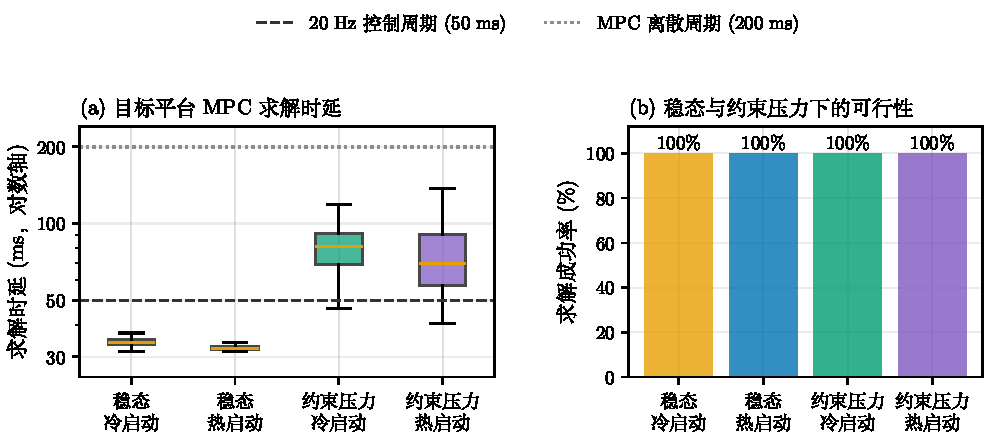
\includegraphics[width=0.96\linewidth,height=0.40\textheight,keepaspectratio,alt={Jetson Orin NX 稳态与约束压力档 MPC wall time 分布及求解成功率}]{../real_experiments/jetson_realtime/figures/jetson_mpc_latency_and_success.pdf}
\caption{Jetson Orin NX 上 MPC 稳态与约束压力档的求解 wall time 分布及成功率（25 W、8 核；求解器微基准）}\label{fig:ch05-jetson-mpc-realtime}
\end{figure}
\FloatBarrier

同一短时 clean run 共记录 60 个整机资源样本，覆盖 30.224 s；CPU mean/p95/max 为 39.9\%/60.0\%/75.1\%，内存 mean/max 为 4838.2/4918.6 MiB，最高温度为 57.4\textdegree C，0.5 s 采样间隔的 p95 为 0.505 s。CPU 分阶段均值为 idle/steady/stress=34.3\%/42.6\%/38.3\%。这些 CPU/GPU、内存和温度是 Jetson 整机遥测，不是求解器进程独占归因；空闲段本身仍含桌面负载。第~\ref{sec:ch05-5-3-1}节 已完成当前容器--真实 PC104 拓扑的 30 min 通信与控制软件栈稳态，但未记录 Jetson 的温度、频率和功耗遥测，故不能替代目标机 thermal soak。

通信侧 4504 个有效上行到达间隔的 p50/p95/p99 为 58.005/85.721/86.095 ms。帧号审计中的 1501 次零增量是重复状态帧，而非 1501 帧丢失；大于 1 的前向跨帧为 0、估算丢帧为 0。first-echo RTT 与求解 wall time 来自不同执行路径，仍不得相加为 ADC--EKF--行为树--控制--PC104 的完整端到端时延。当前结果关闭的是目标平台求解器短时可运行性、真实 PC104 正常通信与固件回显、PC104 故障到行为树的同步零执行器触发链，以及当前拓扑 30 min 稳态；尚未关闭真实 ADC/DVL 输入下的完整调度、Jetson thermal soak 或 Jetson--PC104 单向物理时延。这些边界集中收束于第~\ref{sec:ch05-5-6}节，后续刻度见第~\ref{sec:ch06-6-3}节。

\subsection{故障注入自救逻辑验证}\label{sec:ch05-5-3-4}

故障注入自救逻辑采用等价规则完成统计对照：1000 次持续漏水用于响应延迟，100 条阈值噪声序列用于颤振，500 次低电压、漏水和近底穿越组合故障用于遗漏与死锁判定。两种决策架构均保持 100 ms 紧急响应和 100\% 组合故障生存率，证据只用于决策核心逻辑，不外推为通信链路或执行机构的系统级响应。

\section{综合结果与方法适用性讨论}\label{sec:ch05-5-5-9}

分层实验形成三个相互补充的结论：ES-EKF 在受控退化下维持输出，分源统计揭示协方差失配；UA-MPC 的稳定收益集中于控制平滑与预瞄，横向精度须按场景报告；主动磁横切在单源和可信导航下支持有限横向巡检，深度估计另受场形标定约束。当前限定条件结果见第~\ref{sec:ch05-current-magnetic-closure}节，扰流／输入失配监督与历史 ROS 多横切边界见第~\ref{sec:ch05-inspection-ros-boundary}节，不能跨版本拼接为一次完整验收。

连续运行还受来源时效和调度约束。独立 DDS 接收与分进程短试未通过健康段连续输出门，收到新消息也可能携带过期来源时间。单独 PID 或桥的来源门虽能拒绝旧指令，仍不足以证明目标平台的完整任务连续性。现场验收应在同次记录中连接原始采样、定位、决策、最终目标、PID、UDP 与 PC104 实收，并检查接收时来源年龄、健康段最大空档和故障后持续零命令。实物标定、目标身份、横流误差界、艇体停机包络及目标平台整任务时序尚待验证。

\subsection{证据边界与负结果归因}\label{sec:ch05-5-6}

本节是全章证据边界的索引。磁探测计量、ES-EKF 统计一致性、在线先验几何前提、不确定性感知控制、CBF 与原生因子闭环、实物通信与端到端时延的已完成证据、可写结论与剩余验证，统一列于附录表~\ref{tab:ch05-negative-results}。结果小节仅保留与其结论直接相关的限定。

\section{本章小结}\label{sec:ch05-5-8}

本章验证了三条主线：状态估计在受控退化下保持连续，并以分源统计与鲁棒更新界定观测失配；控制通过预瞄、置信度调制与安全过滤支持近底巡检，收益按层级和场景解释；海缆任务在满足几何前提的数字孪生中恢复先验，v2 在限定条件下完成主动磁观测和有限横向巡检。场形失配、目标身份及执行时效分别决定是否发布深度或继续运动。


实测磁采集与联合反演、Jetson 独立求解器及 PC104 同步零执行器安全链提供了物理锚点。它们支持测量链、部署接口和故障状态传导的可实现性；整机计量、真实输入整任务时序与水域运动仍须独立验收。各项证据边界集中见附录表~\ref{tab:ch05-negative-results}。
